\chapter{The SMELLIE Calibration System}\label{chap:smellie_hardware}
\epigraph{\textit{There's a certain Slant of light,\\
Winter Afternoons ---\\
That oppresses, like the Heft\\
Of Cathedral Tunes ---}}{\textsc{Emily Dickinson}}

As mentioned in Section~\ref{sec:eo_calibs}, one of the principal systems for calibrating the optics of the SNO+ detector is SMELLIE. This calibration device consists of 5 different optical wavelength lasers able to be fired through 15 optical fibres, whose endpoints are attached to the PSUP. A collimator is attached at the end of each fibre, ensuring the emitted light forms a narrow beam across the detector. A diagram of SMELLIE in the detector is shown in Fig.~\ref{fig:smellie_diagram}.

\begin{figure}
    \centering
    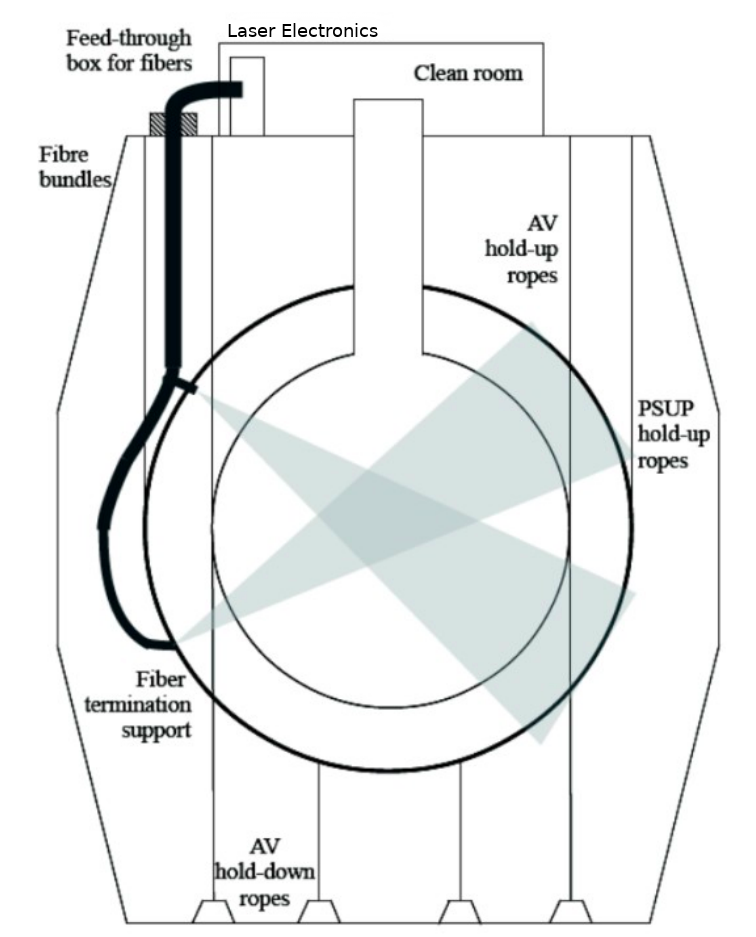
\includegraphics[width=0.48\textwidth]{3_SMELLIEHardware/images/SMELLIE_picture_corrected.png}
    \caption[Diagram of the SMELLIE calibration system within SNO+]
    {Diagram of the SMELLIE calibration system within SNO+. Modified from~\cite{sinclairPositioningTimingCalibration2015}.}
    \label{fig:smellie_diagram}
\end{figure}

The primary goal of SMELLIE is the measurement and monitoring of optical scattering within the detector over the lifetime of the experiment. By firing light from SMELLIE into the detector, some fraction of the photons will be scattered by the detector medium, a fraction of those scattering at large angles relative to the direction of the SMELLIE beam. This strongly scattered light can be detected by PMTs far from the `beamspot', and will also arrive substantially later than light which travelled directly from the fibre to those PMTs. By isolating this scattered light signal, and comparing the quantity observed in data to equivalent simulations with varying scattering lengths, in principle one can measure the detector medium's scattering length. If one takes SMELLIE data with various wavelengths of light at various points in time, one can get a dynamical picture of the optical scattering in SNO+. An analysis of optical scattering in the scintillator phase is made in Section~\ref{sec:scattering_analysis}.

Another substantial measurement that can be made with SMELLIE is the extinction length of the detection media as a function of wavelength and time. This can be done by comparing the fraction of light emitted by the fibre that gets observed in the beamspot after passing through the detector. Section~\ref{sec:ext_length_analysis} covers this analysis in the scintillator phase. Once measurements of both the scattering length and extinction length have been made, it is then possible to derive the absorption length from Eq.~\ref{eq:ext_length_def}.

Both the scattering and absorption lengths of the detector medium impact the propagation of light from physics events, and hence which PMTs get hit along with the times of those hits. If these lengths are systematically off within simulation, this can lead to negative consequences for reconstructing events. In particular, for the scintillator phase, if there is more optical absorption occurring than expected, then because not all absorbed light is re-emitted a larger fraction of photons are lost. Therefore, because energy reconstruction is strongly dependent on the number of PMT hits observed in an event, the energy of events will be systematically under-estimated. Alongside this, light that is re-emitted will only do so after some time delay, and the direction of this re-emission unlikely to be in the same direction as before. This leads to systematic changes in the observed time residual distributions, impacting position reconstruction, as well as any classifiers that use the time residual distribution.

If there is more optical scattering than expected within the scintillator, this also indirectly leads to a greater loss of light because of the increased path length that a photon will typically have to travel before being detected. By consequence, there will be a second-order impact on the energy reconstruction from systematics in the scattering length. Much like changes in the quantity of re-emitted light, increasing the amount of scattering will also systematically effect the position reconstruction and many classifiers.

% \begin{itemize}
%     \item Basic principle for how SMELLIE works: firing collimated laser light into detector to observe scattering events.
%     \item Analysis will measure and monitor scattering in a detector with changing optics.
%     \item One can try and measure some component of this: the cross-section/scattering length versus wavelength and time, and/or the relative scattering length versus wavelength and time.
% \end{itemize}
% [1 page]

A full description of the initial hardware setup of SMELLIE that was used during the air fill and early parts of the water fill phase can be read in~\cite{majumdarMeasurementOpticalScattering2015,cavalliSMELLIEHardwareManual2016}. % cite Krish & DocDB #3511
Since then, a series of hardware upgrades have been made, with~\cite{turnerMeasurementScatteringCharacteristics2022,langrockMeasurementRayleighScattering2016} % cite Esther (+more?)
covering the hardware status used in data taken throughout the water phase.
Fig.~\ref{fig:smellie_timeline} shows a timeline of the hardware upgrades as well as some of the calibration data taking campaigns performed using SMELLIE. The current layout of the SMELLIE hardware, showing the connections between each of the devices within the system, can be seen in Fig.~\ref{fig:smellie_diagram_detailed}. This chapter briefly summarises the current contents of the calibration system, along with descriptions of the major hardware changes made since the water phase.

\begin{figure}
    \centering
    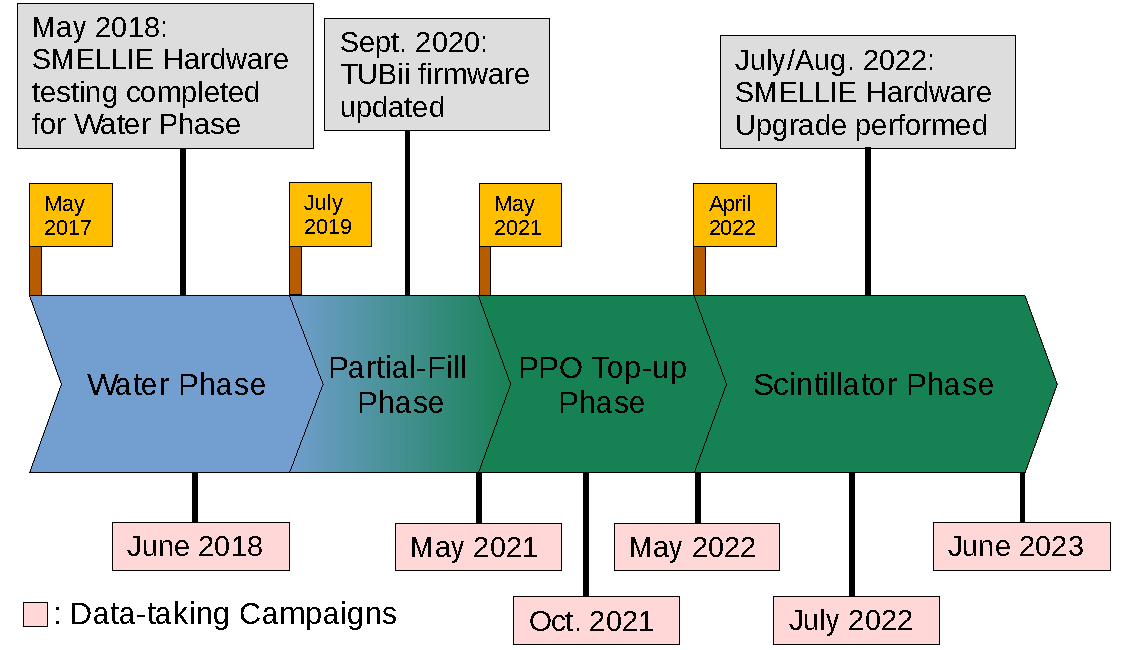
\includegraphics[width=\textwidth]{3_SMELLIEHardware/images/smellie_timeline.pdf}
    \caption[A brief history of SMELLIE hardware work and data-taking campaigns]
    {A brief history of the SMELLIE hardware work and calibration data-taking campaigns of interest for this thesis.}
    \label{fig:smellie_timeline}
\end{figure}

\begin{figure}
    \centering
    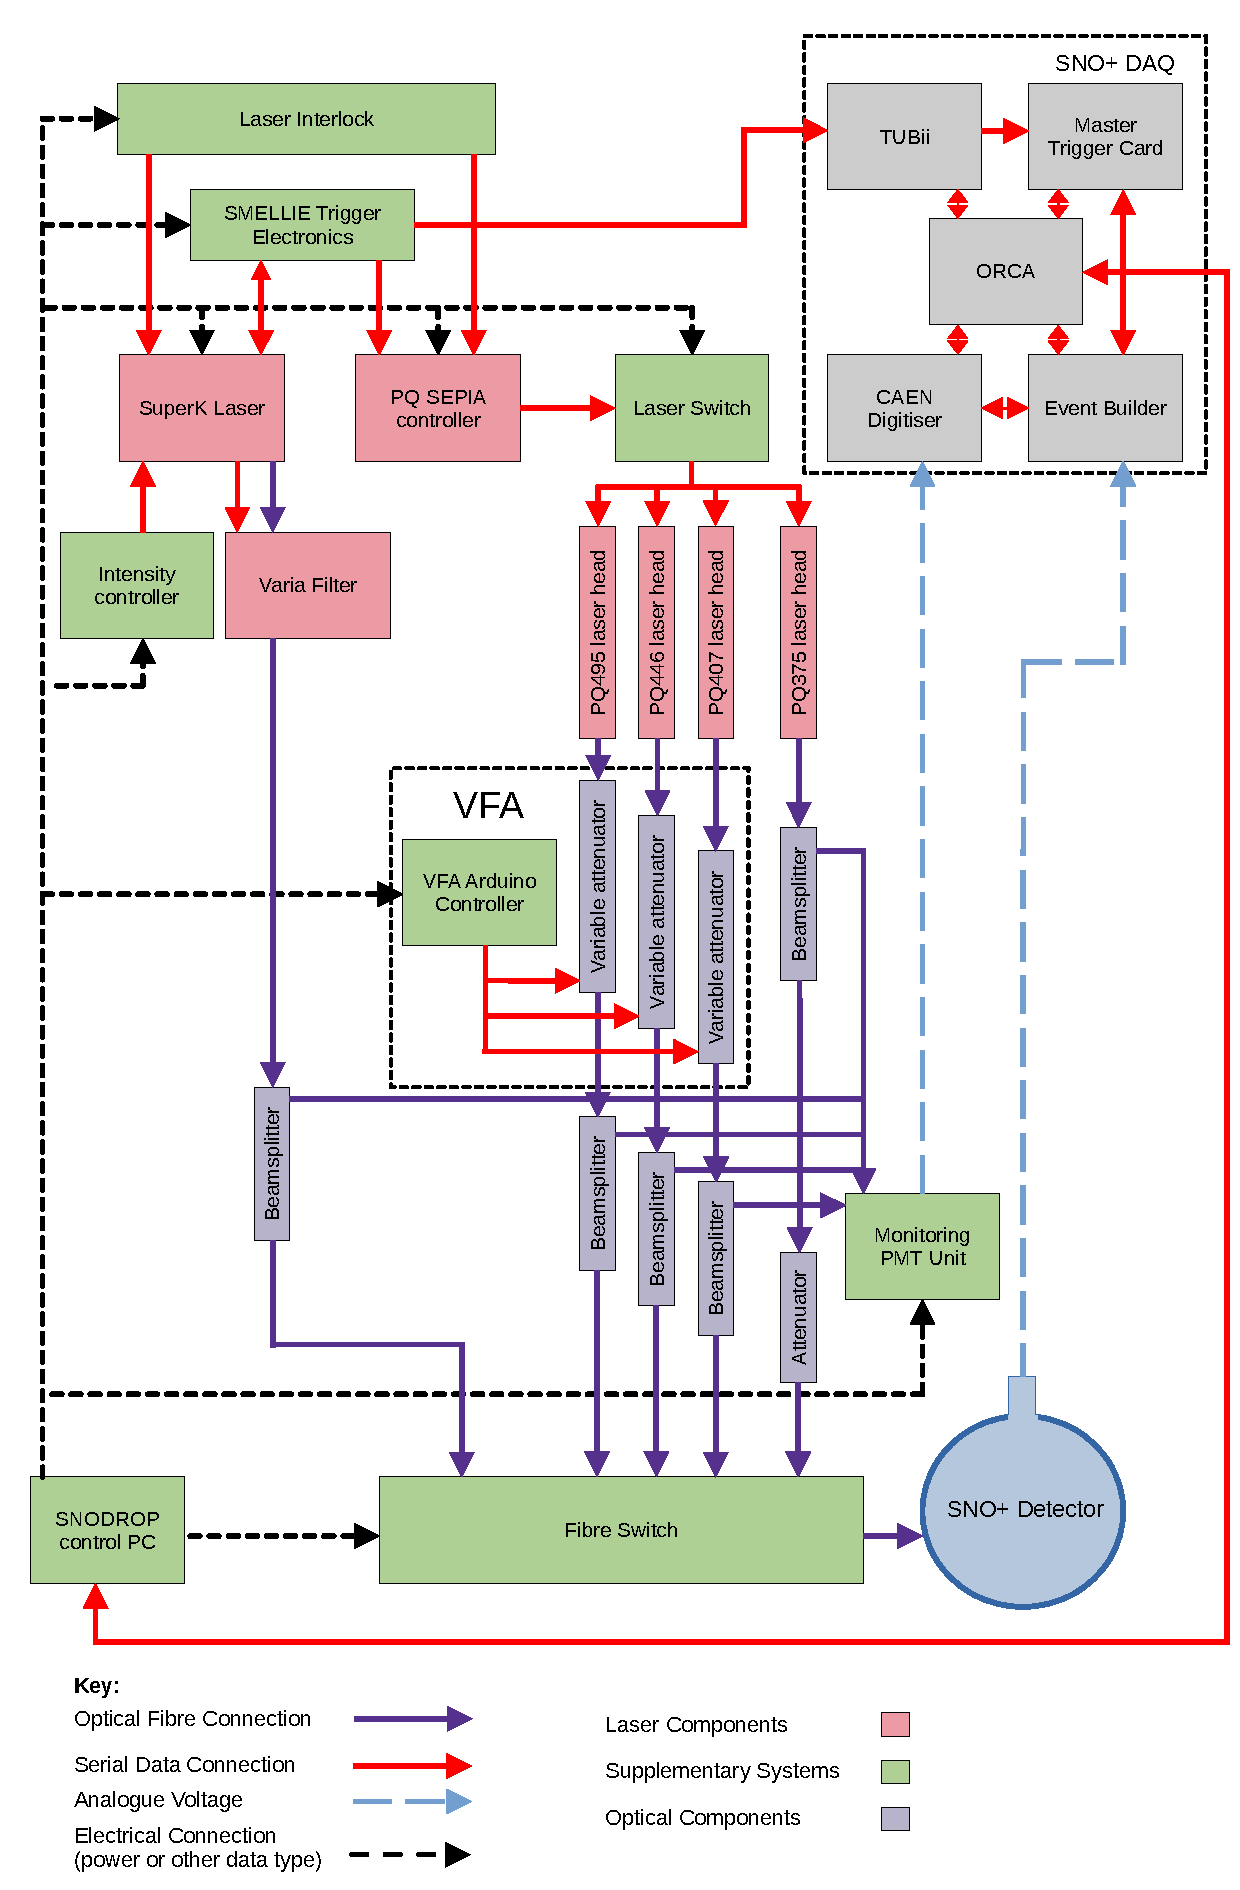
\includegraphics[width=0.95\linewidth]{3_SMELLIEHardware/images/smellie_hardware_schematic.pdf}
    \caption[Diagram of the connections between the various bits of SMELLIE hardware and the rest of the SNO+ detector]
    {Diagram of the connections between the various bits of SMELLIE hardware and the rest of the SNO+ detector, after the changes made in the Summer of 2022. Adapted from~\cite{turnerMeasurementScatteringCharacteristics2022}.}
    \label{fig:smellie_diagram_detailed}
\end{figure}

\section{Lasers}\label{sec:smellie_lasers}
\nomenclature{\textbf{PQ}}{PicoQuant}
Fundamental to the SMELLIE calibration system are 5 optical-wavelength lasers. Four of these are fixed-wavelength pulsed-diode laser heads from the company PicoQuant. These `PQ' laser heads each emit with a different narrow wavelength spectrum, peaking at \SI{375}{\nm}, \SI{407}{\nm}, \SI{446}{\nm}, and \SI{495}{\nm}. These are referred to as the PQ375, PQ407, PQ446, and PQ495 lasers, respectively. In addition to these lasers, a SuperK Compact laser made by NKT Photonics (hereafter referred to as the SuperK laser) is also used\footnote{
    Apologies to those more familiar with `SuperK' referring to the SuperKamiokande experiment based in Japan: this laser bears no relation.
}. Unlike the PQ laser heads, the SuperK is a super-continuum laser able to produce laser light over the whole optical wavelength spectrum. Because the interest is almost always in determining optical properties at specific wavelengths, a variable bandpass filter also built by NKT Photonics known as the SuperK Varia has been included. This allows the user to select any wavelength interval between \SIrange{400}{700}{\nm}, with a minimum bandwidth of \SI{10}{\nm}. The wavelength and emission timing characteristics of all five lasers are shown in Fig.~\ref{fig:smellie_emission_wav_timing}. The $\mathcal{O}(\SI{1}{\ns})$ time widths for the lasers are essential for scattering analyses as they allow for much greater precision in knowing when photons should arrive at PMTs in the detector than with an LED source. This is why SMELLIE uses lasers for its light generation, unlike the LEDs used for AMELLIE and TELLIE.

\begin{figure}
    \centering
    \begin{subfigure}{0.98\textwidth}
        \centering
        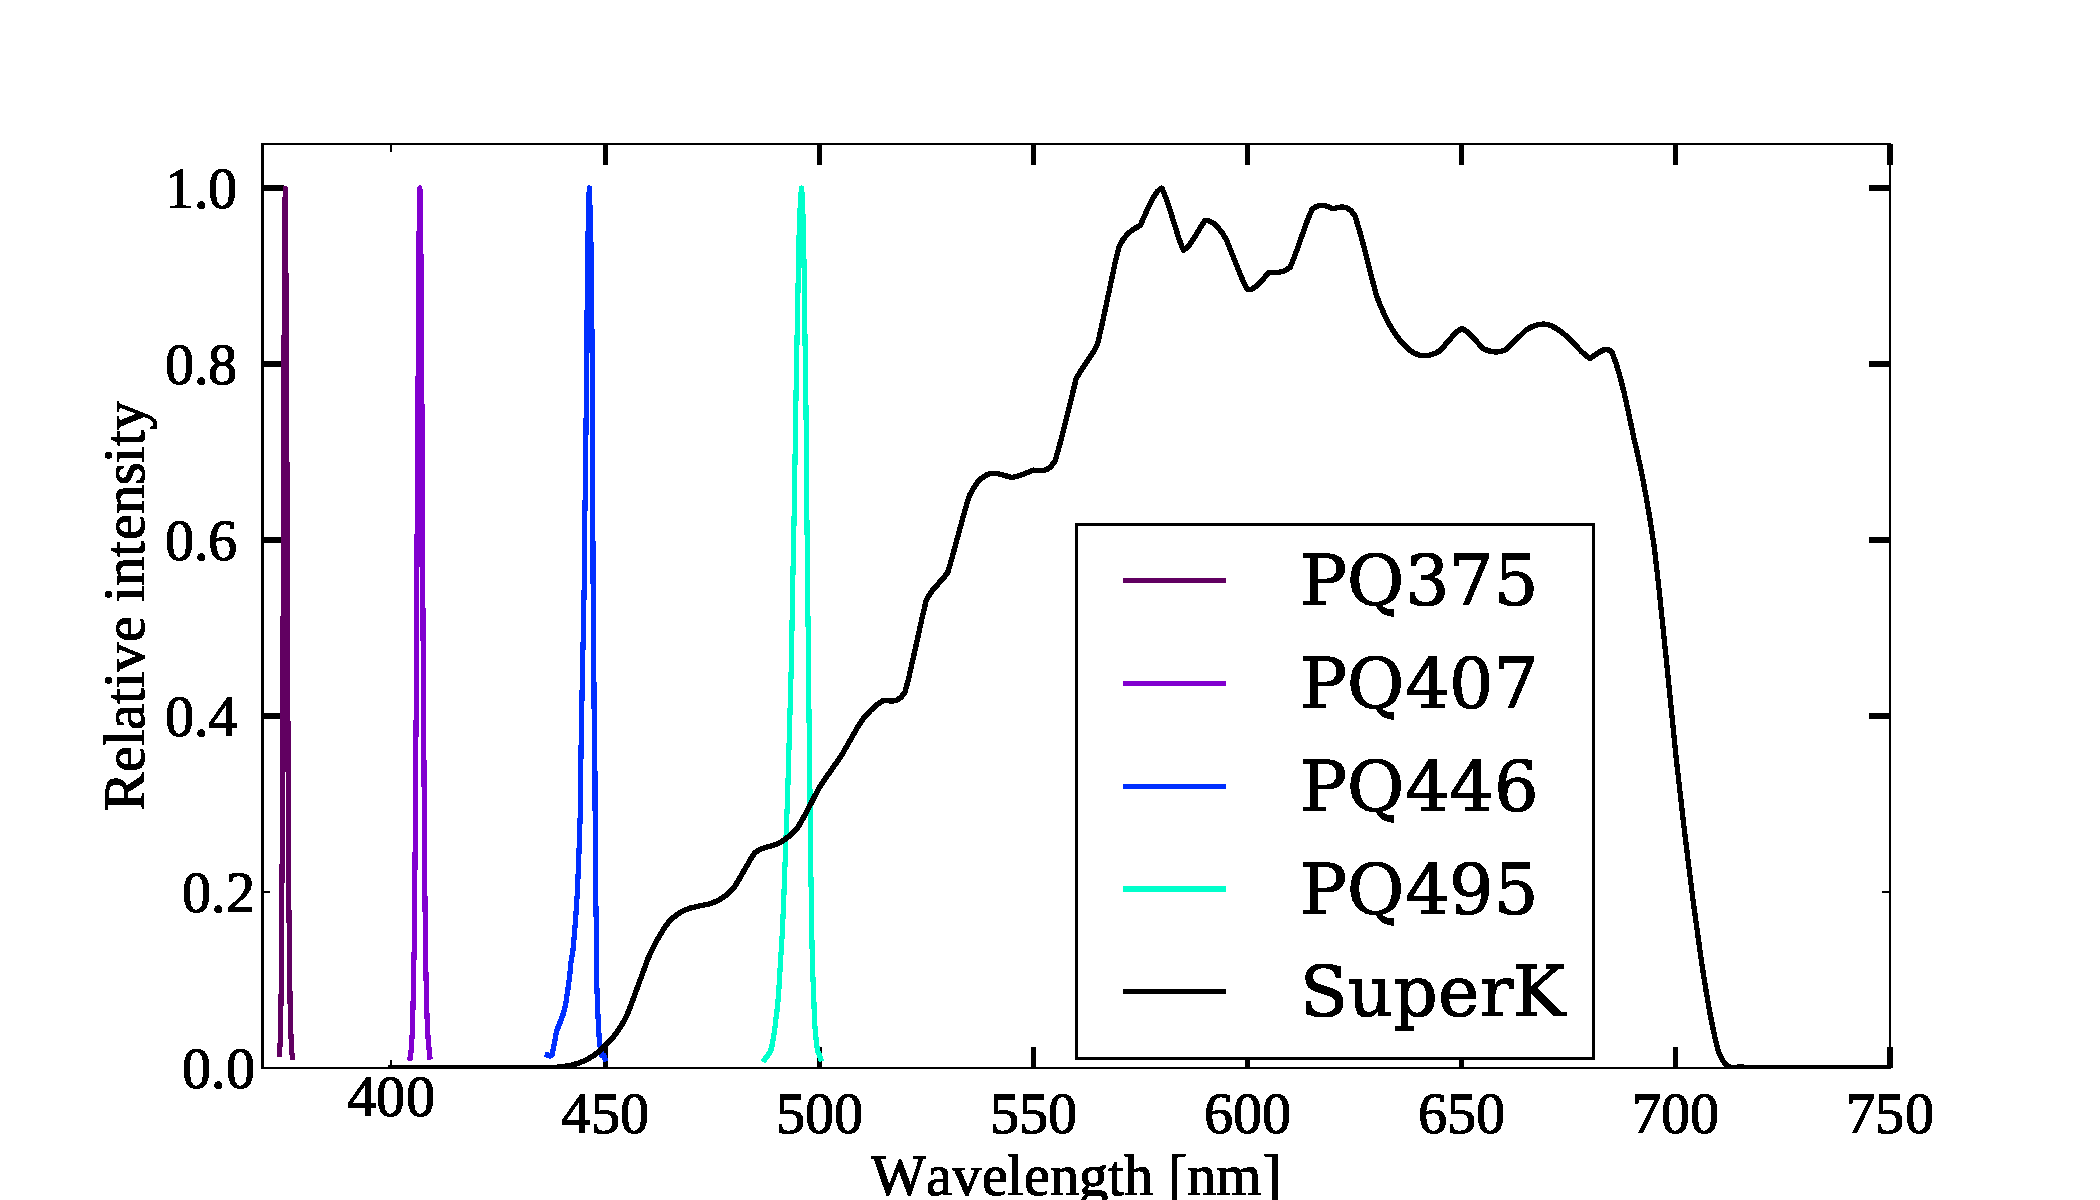
\includegraphics[width=0.98\textwidth]{3_SMELLIEHardware/images/smellie_laser_wavelengths.pdf}
        \caption{}
        \label{fig:smellie_emission_wavelengths}
    \end{subfigure}
    \begin{subfigure}{0.98\textwidth}
        \centering
        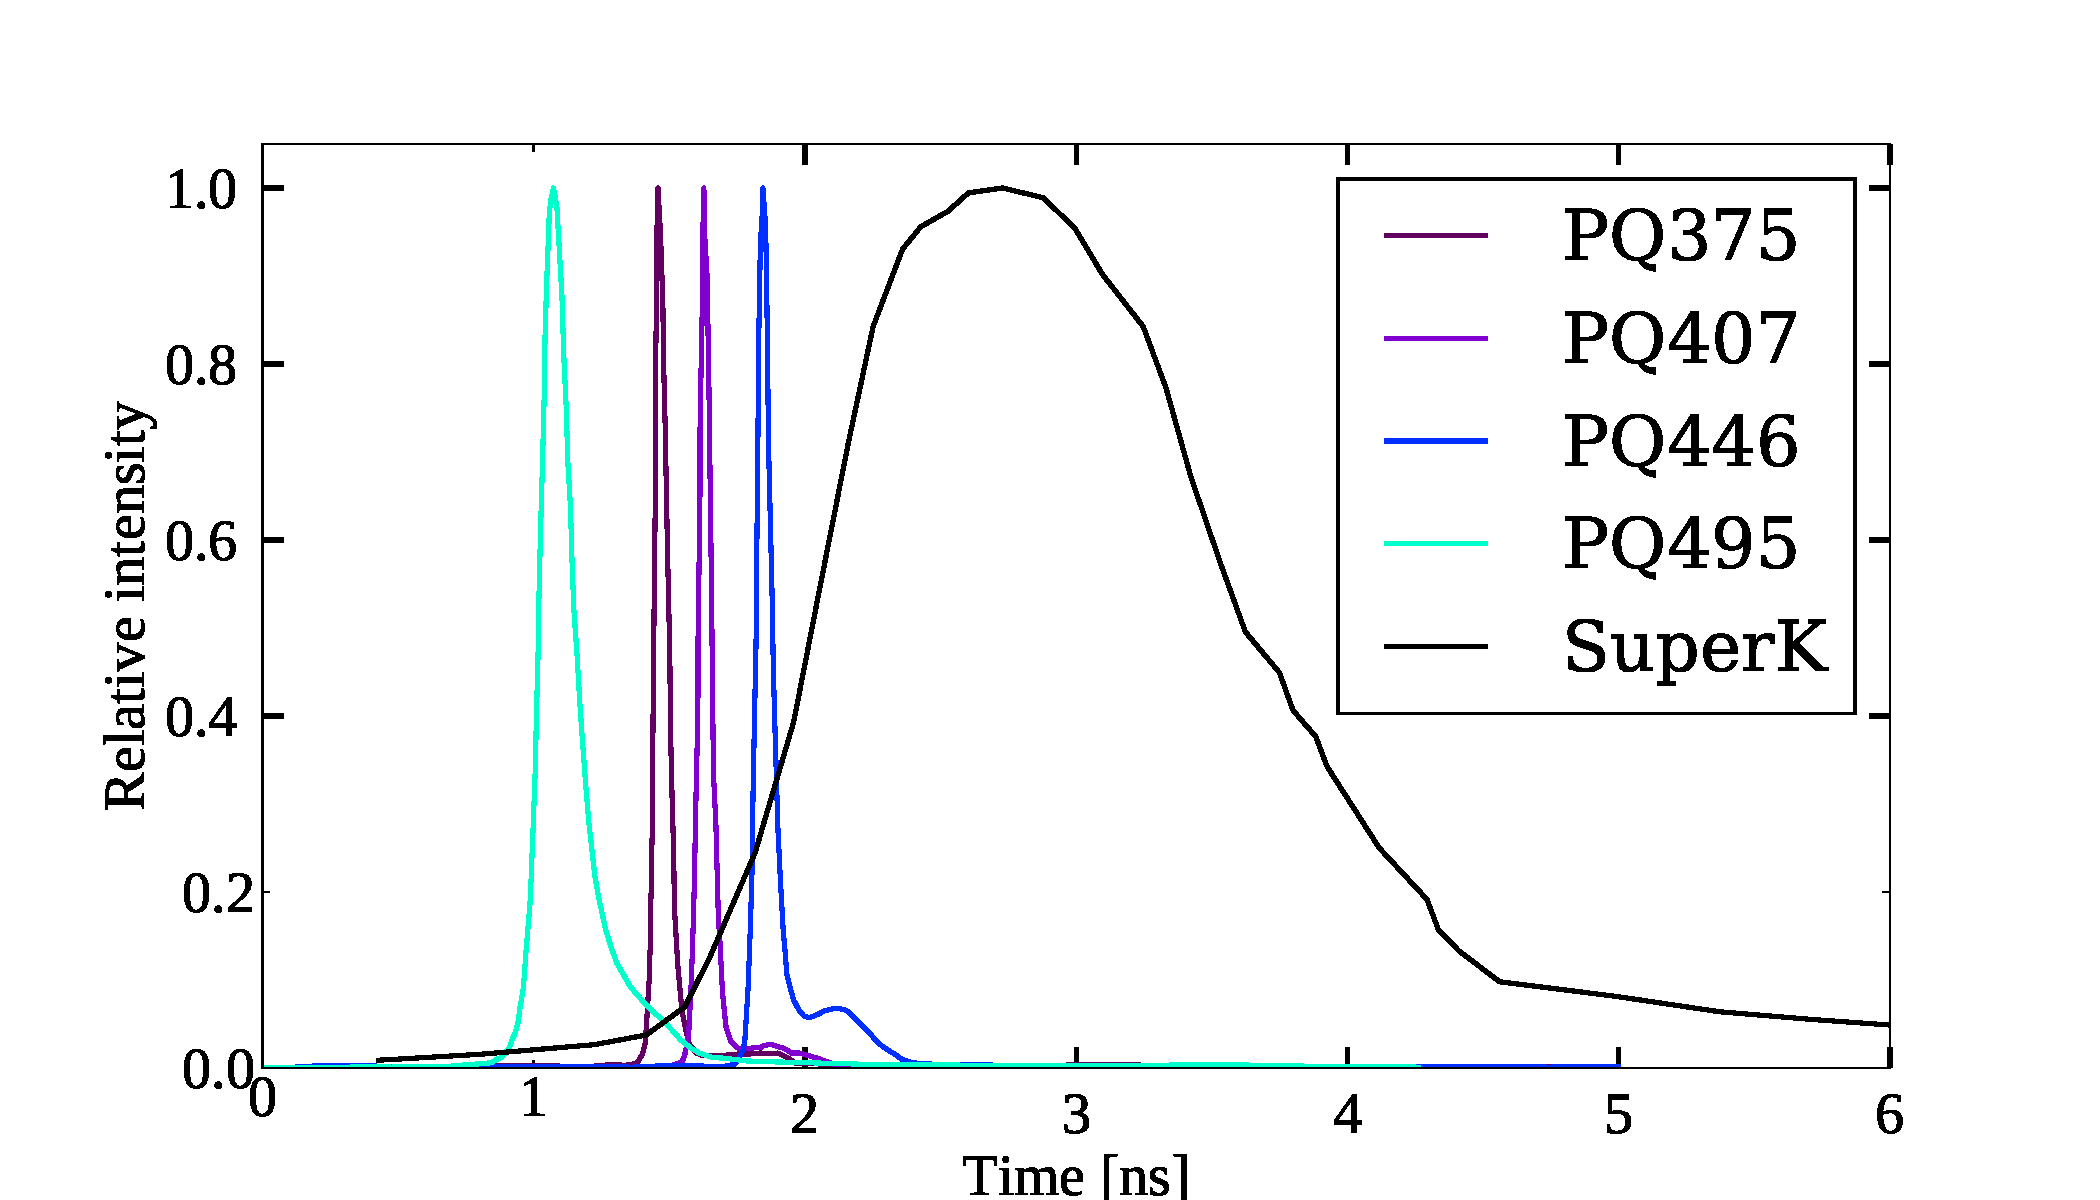
\includegraphics[width=0.98\textwidth]{3_SMELLIEHardware/images/smellie_laser_timings.pdf}
        \caption{}
        \label{fig:smellie_emission_timing}
    \end{subfigure}
    \caption[Emission wavelength and timing spectra of the lasers used in SMELLIE]
    {Emission wavelength (a) and timing (b) spectra of the lasers used in SMELLIE. PQ spectral information taken from the manufacturer; SuperK information measured by J. Lidgard~\cite{lidgardSupercontinuumAdditionSMELLIE2018}.}
    \label{fig:smellie_emission_wav_timing}
\end{figure}

\section{Controlling Laser Intensities}\label{sec:smellie_attenuators}
It is important to be able to control the quantity of light that enters the detector from a given pulse of one of the lasers. This is done in two parts. For the SuperK laser, the raw power of the beam in a pulse can be set as a percentage of the maximum possible power for that wavelength. Once a light pulse has been generated, it is then attenuated by a neutral density filter contained within the SuperK laser hardware.

For the PQ lasers, a PicoQuant-brand SEPIA II laser driver is used to set the raw pulse intensity and firing rate. Unlike the SuperK, the intensity control is given by the laser driver's driving voltage, as a fraction of the maximum possible voltage. For both types of laser, the driving voltage is given as a number between 0 and 1000, where 1000 indicates the maximum allowed driving voltage for that laser. Problematically, the dependence on the raw output intensity of the PQ laser heads are highly nonlinear with respect to the amplitude of the driving voltage. To demonstrate, consider the observed fraction of events in which each PMT was hit. This is known as the PMT occupancy, and the maximum PMT occupancy is shown as a function of driving voltage for SMELLIE events using the PQ lasers in Fig.~\ref{fig:pq_old_intensity_dependence}.

For low driving voltages, the resulting maximum PMT occupancy is very small, and rises slowly. However, near the `lasing threshold' the occupancy observed rapidly climbs. Above this threshold, some PMTs in the beamspot `saturate', having an occupancy of 1. As will be seen in Chapter~\ref{chap:beam_profiling}, information about the light intensity incident on a given PMT can be derived in a straightforward manner only if the light level is stable for a given set of data, and the occupancy on the PMT is below 1. When driving a laser head near its lasing threshold the shot-to-shot variation in observed light intensity in the detector can also become substantial: see Fig.~\ref{fig:pq_threshold_intensity_variation} for an example of this occurring.

\begin{figure}
    \centering
    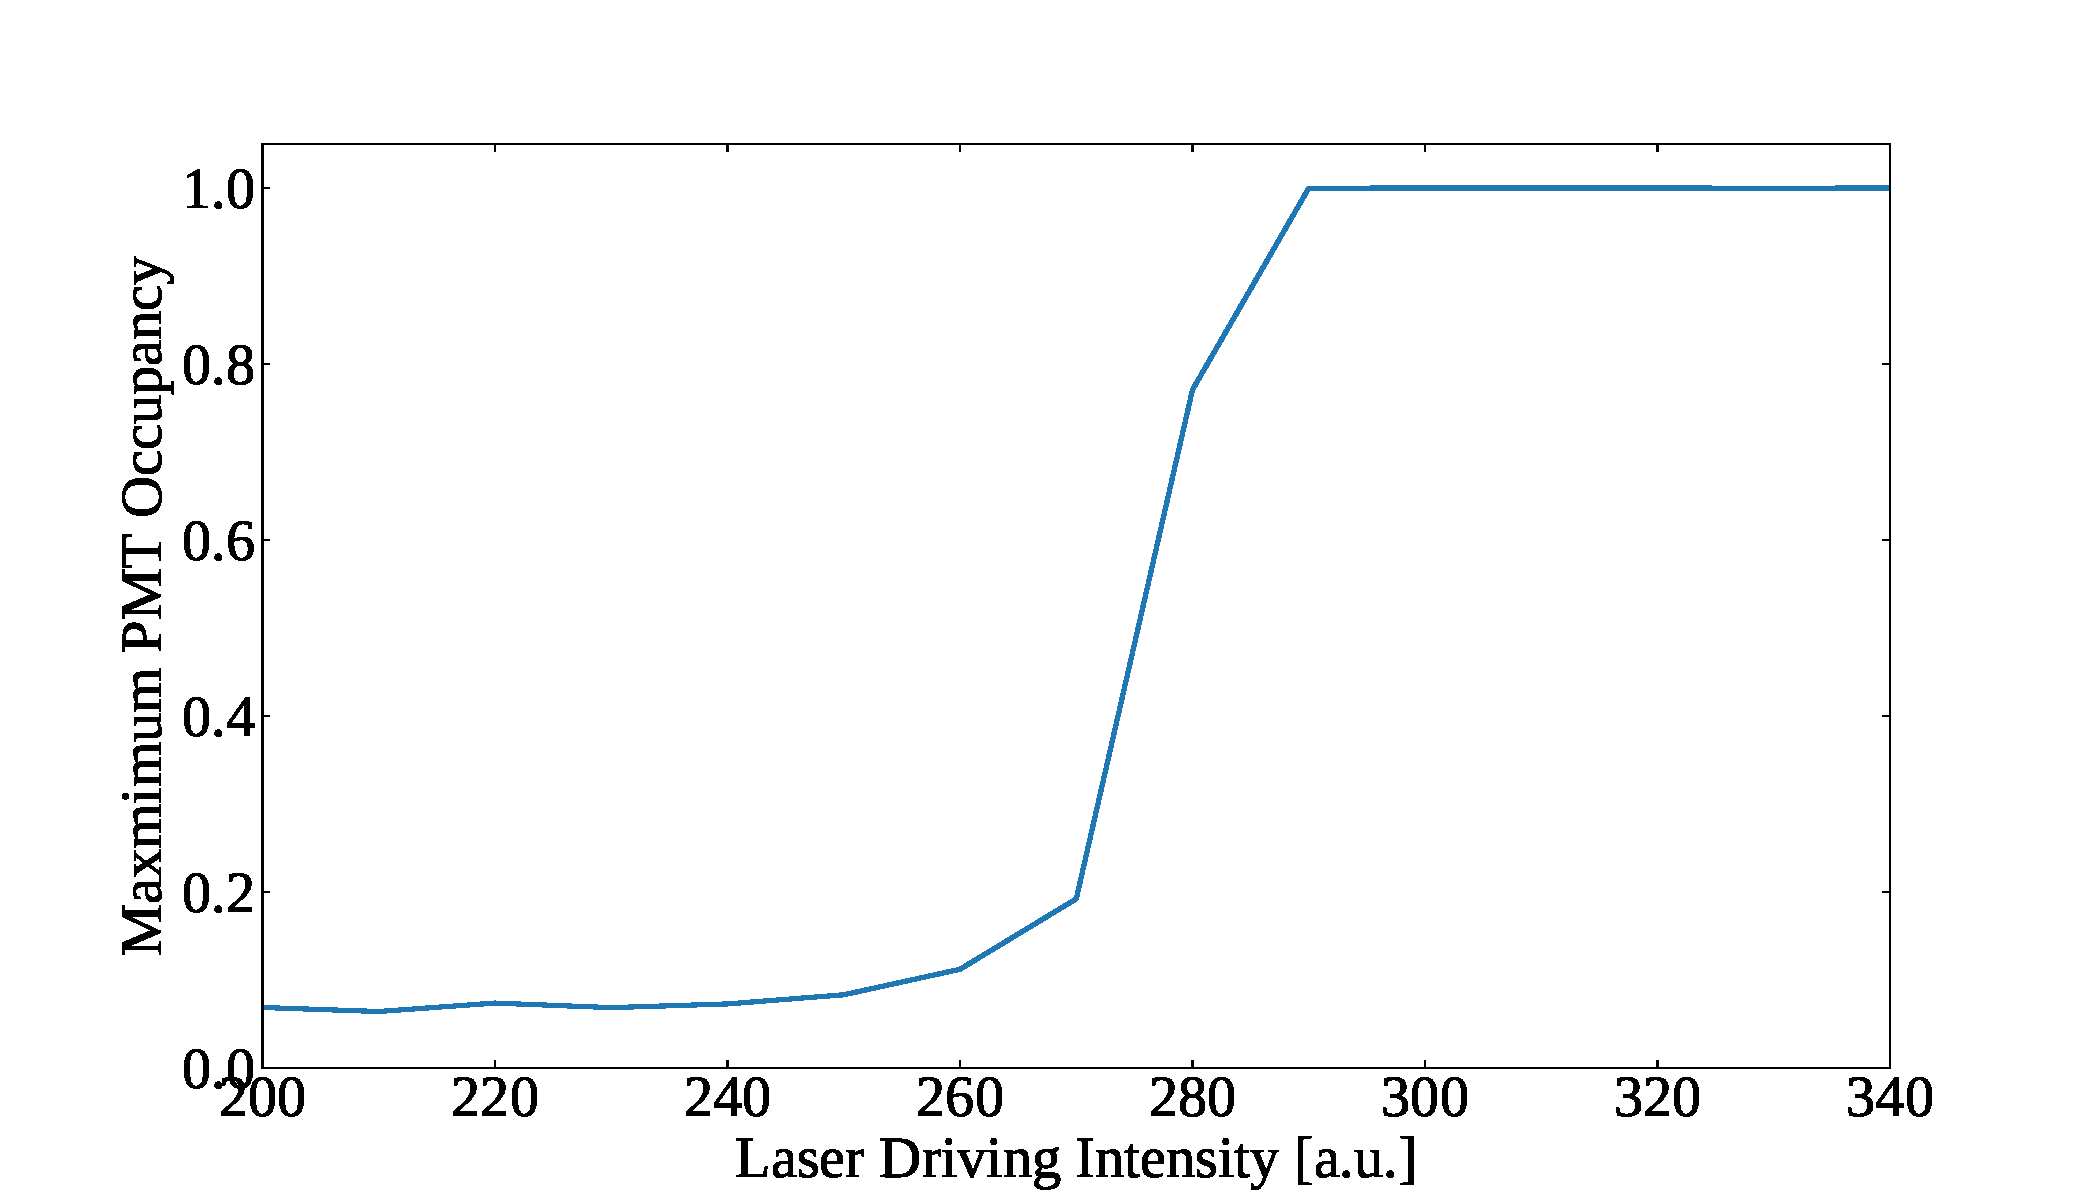
\includegraphics[width=0.8\textwidth]{3_SMELLIEHardware/images/smellie_intensity_scan_pq446_old.pdf}
    \caption[Typical impact of driving voltage intensity for PQ446 laser on observed maximum occupancy in the detector]
    {Typical impact of driving voltage intensity for PQ446 laser on observed maximum occupancy in the detector. Data taken on February 22\textsuperscript{nd}, 2021.}
    \label{fig:pq_old_intensity_dependence}
\end{figure}

\begin{figure}
    \centering
    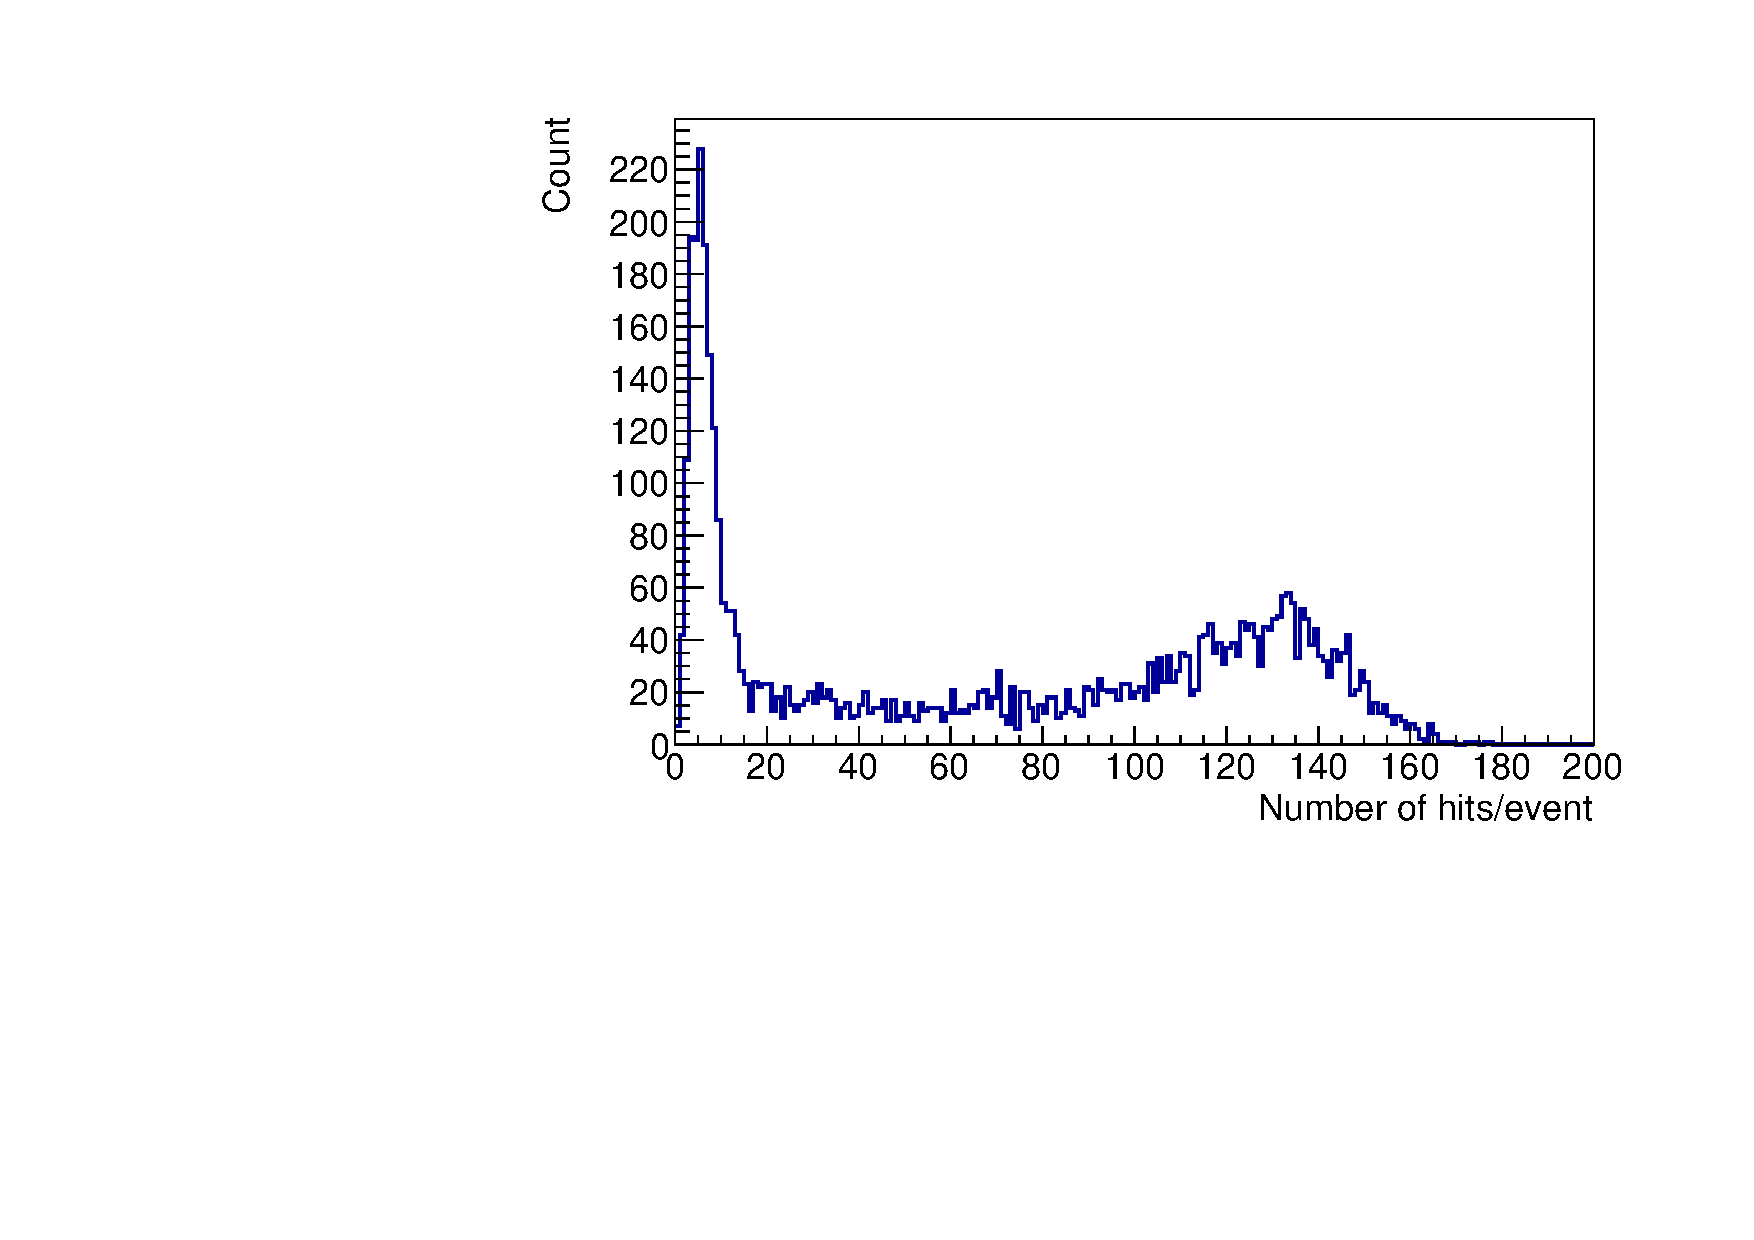
\includegraphics[width=0.8\textwidth]{3_SMELLIEHardware/images/run_268221_8_nhit_dist.pdf}
    \caption[Distribution of the number of PMT hits observed per event for laser PQ446]
    {Distribution of the number of PMT hits observed per event in the detector for laser PQ446 when the driving voltage value is 280. Data taken on February 22\textsuperscript{nd}, 2021.}
    \label{fig:pq_threshold_intensity_variation}
\end{figure}

During the water and scintillator phases up until Summer 2022, some data taken, especially using the PQ407 and PQ446 lasers, suffered from large shot-to-shot intensity variations. Throughout this period, after the light was generated by a PQ laser head it would then be passed through an attenuator, fixed to some nominal attenuation setting for each laser. In theory, one could solve the intensity variation problem by deliberately setting the intensity well beyond the lasing threshold, and then changing the attenuation of the attenuator to obtain the occupancies within the detector one is interested in. However, under the original hardware this was untenable as this would require someone to manually change the attenuations in-person every time a different set of SMELLIE run conditions were proposed.

\nomenclature{\textbf{VFA}}{Remotely-controllable Variable Fibre Attenuator}
Instead, Jeff Lidgard built a piece of hardware called the remotely-controllable Variable Fibre Attenuator (VFA), shown in Fig.~\ref{fig:vfa_picture}. Contained within a metal housing were a `precision variable attenuator' from DiCon Fibreoptics~\cite{diconfibreoptics30dBPrecisionVariable2017} % cite DiCon attenuator specsheet online
for each PQ laser, along with an Arduino running firmware written by J. Lidgard to enable communication with each of the attenuators. Commands could be sent to a given attenuator asking for a specific attenuation expressed as a number between 0 and 3000, where the number divided by 100 gives the theoretical attenuation. Following ex-situ testing by J. Lidgard and Jasmine Simms, the VFA was installed underground by myself and Armin Reichold in July 2022, with some assistance from J. Lidgard in integration of the hardware and SMELLIE server software.

\begin{figure}
    \centering
    \includegraphics[width=0.8\textwidth]{3_SMELLIEHardware/images/VFA_MPU_picture.png}
    \caption[Picture of the VFA during installation into the ELLIE hardware rack]
    {Picture of the VFA during installation into the ELLIE hardware rack. The VFA box rests beneath the fibres connecting to the beamsplitters, as well as the newly-installed Monitoring PMT Unit (see Section~\ref{sec:smellie_mpu} for details).}
    \label{fig:vfa_picture}
\end{figure}

During testing of the VFA in-situ, it was discovered that the actual attenuation of the variable attenuator at the minimum setting of \SI{0}{\dB} for the PQ375 laser was so strong that negligible light was ever observed in the detector. This is likely because the precision variable attenuator components were primarily designed by the manufacturer with infrared fibre-optic transmission in mind. Because of this, the PQ375 was not hooked up to the VFA, and kept its original attenuator setup. After fixing the driving voltage settings for PQ407, PQ446, and PQ495 to be 1000, 750, and 750 respectively, % add in numbers!
the observed maximum PMT occupancy in the detector was once again compared to the input laser intensity setting. For PQ375 this input parameter remained the driving voltage; for the others, the attenuation setting was now used. The results can be seen in Fig.~\ref{fig:pq_new_intensity_dependence}. As hoped for, the three PQ lasers hooked up to the VFA can now have stable intensities of light observed in the detector over multiple orders of magnitude of observed intensity.

\begin{figure}
    \centering
    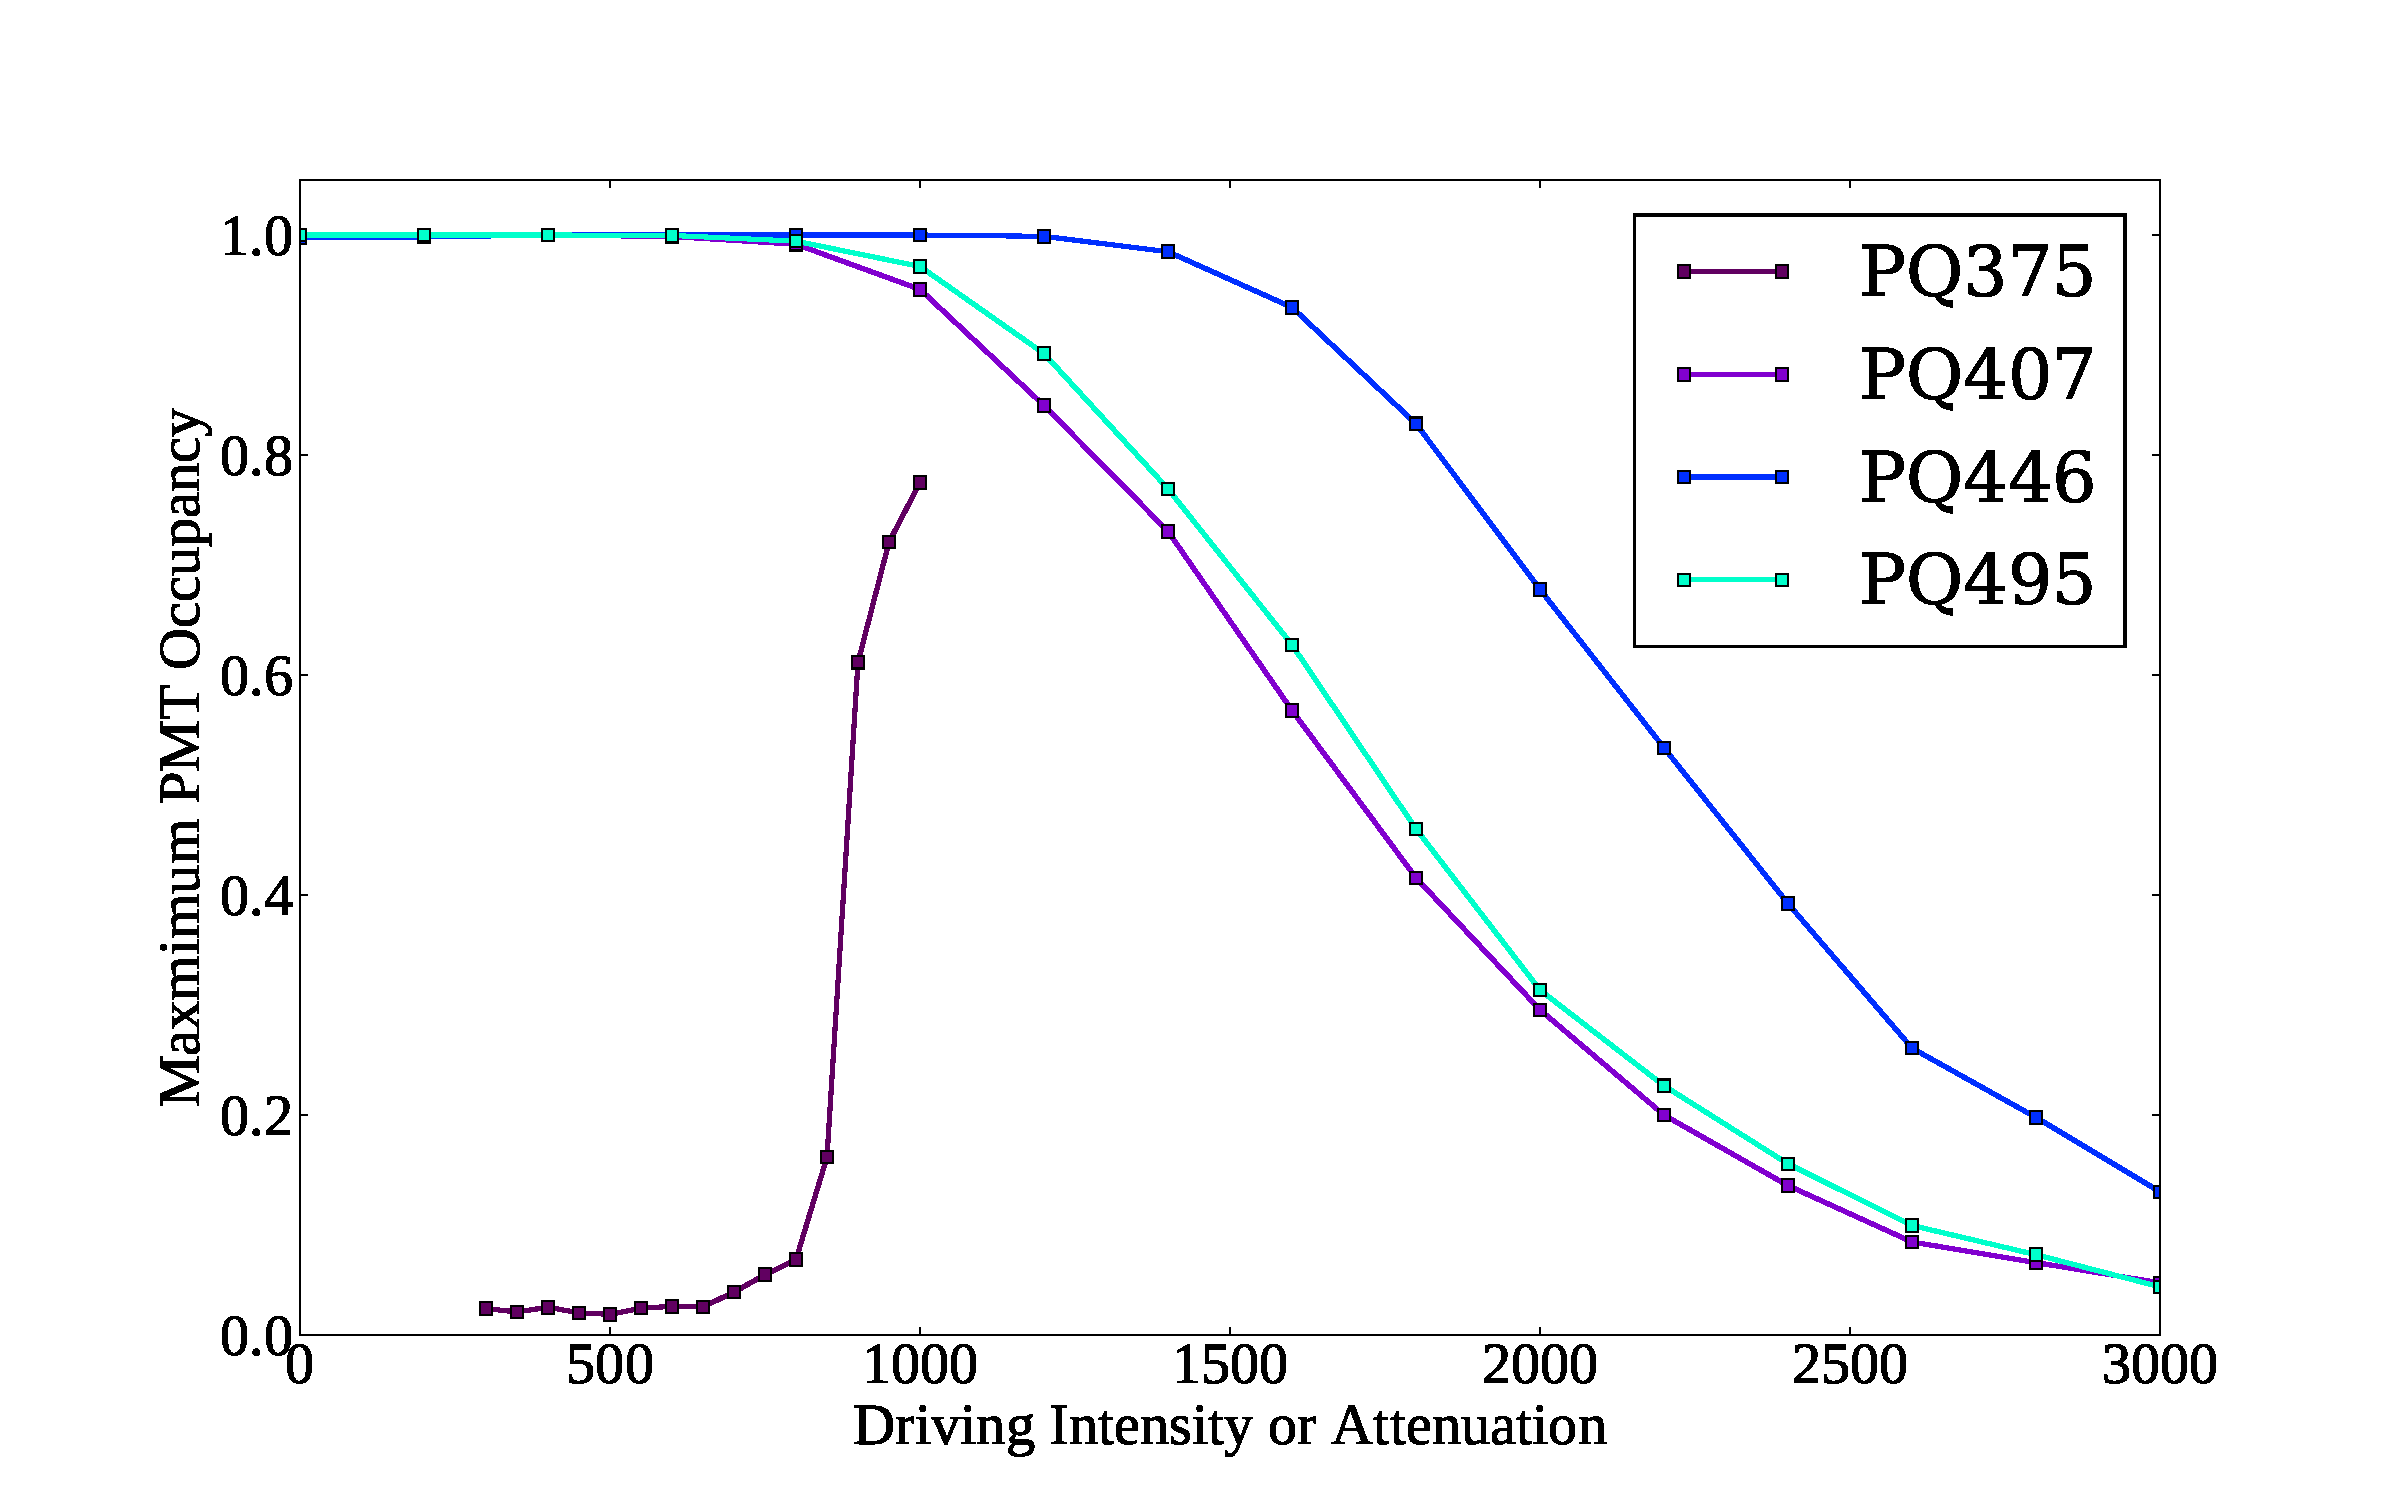
\includegraphics[width=0.8\textwidth]{3_SMELLIEHardware/images/smellie_intensity_scan_new.pdf}
    \caption[Maximum occupancy in the detector as a function of the attenuation parameter value used]
    {Maximum occupancy in the detector as a function of the attenuation parameter value used, for each of PQ407, PQ446, and PQ495. Because PQ375 is not plugged into the VFA, its dependence on the driving intensity is shown instead. Data taken on the 12\textsuperscript{th} of January, 2023.}
    \label{fig:pq_new_intensity_dependence}
\end{figure}

\section{Propagation of Light into the Detector}\label{sec:smellie_fibres}
Once a pulse of optical light has been generated by the lasers and attenuated to the desired intensity, the next step is to navigate that light into the detector. This is achieved through a network of Corning-brand ``InfiniCor SXi'' multimode optical fibres~\cite{corningCorningInfinicor502007}. % cite Corning datasheet(s)
These fibres were chosen in part for their low intrinsic radioactivity~\cite{clarkELLIEFibreRadioactivity2011}, % cite Radon Assay/Krish's thesis
as well as having a graded index as a function of radius. This latter property enables lower dispersion between different modes of the light, so that the initial sharpness of any given light pulse in time is maintained. However, because these fibres were mainly designed for telecommunication purposes, their nominal operating wavelengths are out in the near-infrared, \SIrange{750}{1450}{\nm}. As SMELLIE only fires wavelengths in the range \SIrange{375}{700}{\nm}, there is a small but non-negligible amount of light lost when propagating through the fibres.

After some light is split off by a beamsplitter to allow for ex-situ monitoring of the light pulse (see Section~\ref{sec:smellie_mpu}), it is sent to the Fibre Switch, two boxes manufactured by Laser Components UK that allows a user to remotely-control which of the fibres to send the light down into the detector.

Finally, the light that passes through the fibre switch propagates along one of the 15 optical fibres that have been submerged in the SNO+ cavity, whose ends are mounted to the PSUP. Specifically, sets of three fibres are mounted to a given node of the PSUP, with associated node numberings: nominally 07, 25, 37, 55, and 21. These provide for a variety of positions within the detector from which light can be emitted. Each mounting which holds three of the optical fibres also contains collimators, designed to reduce the possible range of angles with which the light can be emitted from. This is particularly important for SMELLIE, because unlike the other ELLIE systems, a thin `pencil' beam of light across the detector is ideal for measuring scattering~\cite{majumdarMeasurementOpticalScattering2015}. % cite Krish.
The mounting also points each of the three fibres in different directions: \ang{0}, \ang{10}, and \ang{20} from the direction radially towards the centre of the detector.

Each fibre is given a name that nominally refers to both its mounting position and its pointing direction. For example, the label `FS107' corresponds to the SMELLIE fibre mounted at node 07 with a pointing direction of \ang{10}. Unfortunately, during installation some fibres were mislabelled, leading to the node mounting points and pointing directions of some fibres being inconsistent with the labelling convention. The actual mounting nodes and pointing directions for each fibre can be seen in Table~\ref{tab:smellie_fibre_labellings}.
The 3D positions and pointing directions of all the fibres are determined in~\cite{langrockMeasurementRayleighScattering2016}, and shown in Fig.~\ref{fig:smellie_pos_dirs}.

\begin{table}
    \centering
    \begin{tabular}{c c c}
        \hline
        Fibre   & Node & Pointing direction \\ \hline \hline
        FS007   & 07   & \ang{0}  \\
        FS107   & 07   & \ang{10} \\
        FS207   & 07   & \ang{20} \\
        FS025   & 25   & \ang{0}  \\
        FS125   & 25   & \ang{10} \\
        FS225   & 25   & \ang{20} \\
        FS037   & 37   & \ang{10} \\
        FS137   & 37   & \ang{0}  \\
        FS237   & 37   & \ang{20} \\
        FS055   & 55   & \ang{10} \\
        FS155   & 55   & \ang{20} \\
        FS255   & 55   & \ang{0}  \\
        FS093   & 21   & \ang{0}  \\
        FS193   & 21   & \ang{10} \\
        FS293   & 21   & \ang{20} \\
        \hline
    \end{tabular}
    \caption[SMELLIE fibre names, their associated mounting nodes on the PSUP, and their pointing direction.]
    {SMELLIE fibre names, their associated mounting nodes on the PSUP, and their pointing direction. Taken from~\cite{turnerMeasurementScatteringCharacteristics2022}.}
    \label{tab:smellie_fibre_labellings}
\end{table}

\begin{figure}
    \centering
    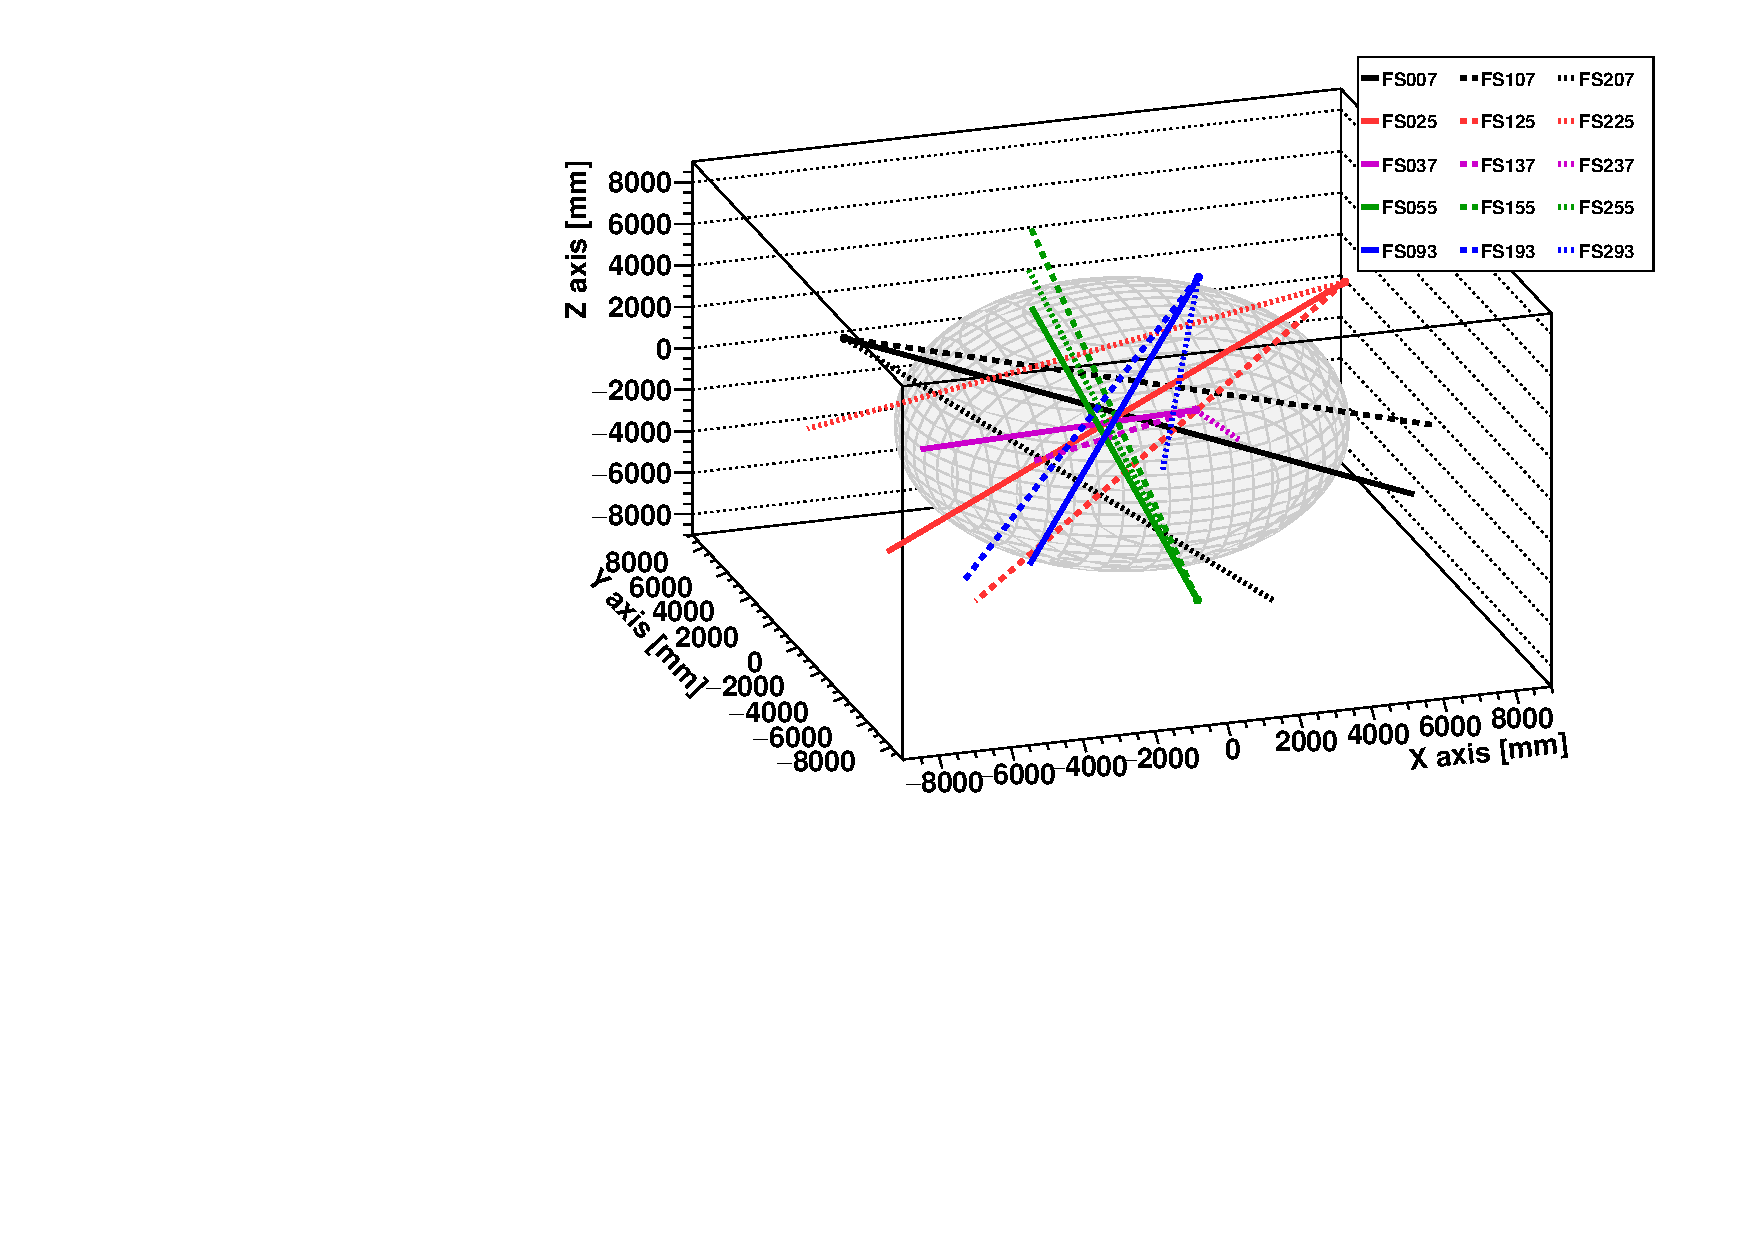
\includegraphics[width=0.8\textwidth]{3_SMELLIEHardware/images/fibre_positions.pdf}
    \caption[Fibre emission points and nominal pointing directions]
    {Fibre emission points and nominal pointing directions within the detector.}
    \label{fig:smellie_pos_dirs}
\end{figure}

When performing analysis with SMELLIE, a fibre-centric spherical-polar coordinate system is used. This coordinate system was first fully-developed by E. Turner; full details can be read in~\cite{turnerMeasurementScatteringCharacteristics2022}. A position $\bm{x}$ is measured relative to a given fibre's mounting position, $\bm{f}$ (hereafter referred to as simply the fibre's position). Polar angles, labelled $\alpha$, are measured relative to the fibre's pointing direction, $\bm{\hat{u}}$. As a result, a line from the fibre position along $\alpha = 0$ across the detector should in theory hit the centre of the fibre's beamspot. Finally, in order to define the azimuthal angle $\phi$, the plane orthogonal to $\bm{\hat{u}}$ is considered. Both $\bm{x}$ and the unit vector in the vertically-upwards direction, $\bm{\hat{z}}$, are projected onto this plane, forming the vectors $\bm{x_{proj}}$ and $\bm{\hat{z}_{proj}}$, respectively. $\phi$ is then defined as the angle going from $\bm{\hat{z}_{proj}}$ to $\bm{x_{proj}}$ if one were to look at the plane in the direction of $\bm{\hat{u}}$. Mathematically, this can be written as:
\begin{equation}
    \tan\phi = \frac{
        \left(\bm{x_{proj}}\times\bm{\hat{z}_{proj}}\right)\cdot\bm{\hat{u}}
        }{\bm{x_{proj}}\cdot\bm{\hat{z}_{proj}}}.
\end{equation}

\section{The Monitoring PMT Unit}\label{sec:smellie_mpu}
\nomenclature{\textbf{MPU}}{Monitoring PMT Unit (for SMELLIE)}
As mentioned in the previous section, part of the light generated by the lasers gets split off from the main fibre path down into the detector, and is used for monitoring purposes. This is achieved with a box known as the Monitoring PMT Unit (MPU). As the name suggests, the MPU contains a small PMT that generates an electronic signal pulse from the laser light. This signal is then shaped by electronics, and passed to the detector's central CAEN digitiser to have that pulse digitised.

One problem with the existing MPU within SMELLIE was that the pulse it produced was so broad that 300 ADC samples were needed to capture the full shape (the CAEN samples at a rate of 1 every \SI{4}{\ns}). This led to a large fraction of data being generated by SMELLIE events coming not from the PMT hit information, but simply the MPU's signal digitisation. A natural consequence of this was the rate at which the lasers could be fired had to be limited to typically \SI{1}{\kHz}, otherwise the detector was not able to handle the rate of data being generated.

Because of this, a new MPU was commissioned. Built by Adam Baird and Johan Fopma from the Oxford Physics Central Electronics Group, this MPU had updated electronics such that the pulse was shaped shorter. In addition, the rise time of the pulse was made faster, in the hopes that the emission time of the light pulse for a given event could be captured more accurately. The new MPU was installed by myself and A. Reichold at the same time as the VFA, in Summer 2022.

Alongside the installation of the new hardware, the settings in ORCA for the CAEN digitisation of the MPU signal were updated. In particular, the number of samples made by the CAEN was shortened from 300 down to 124. The timing of the CAEN sampling and delay on the TUBii trigger (more on the trigger shortly) was also modified. As a result of these changes, a much shorter trace was now being generated, without missing any part of the MPU pulse or moving the observed TAC for hits in the detector outside the trigger window. Fig.~\ref{fig:caen_trace_comparison} shows a comparison between typical MPU pulses taken before and after the upgrades.

\begin{figure}
    \centering
    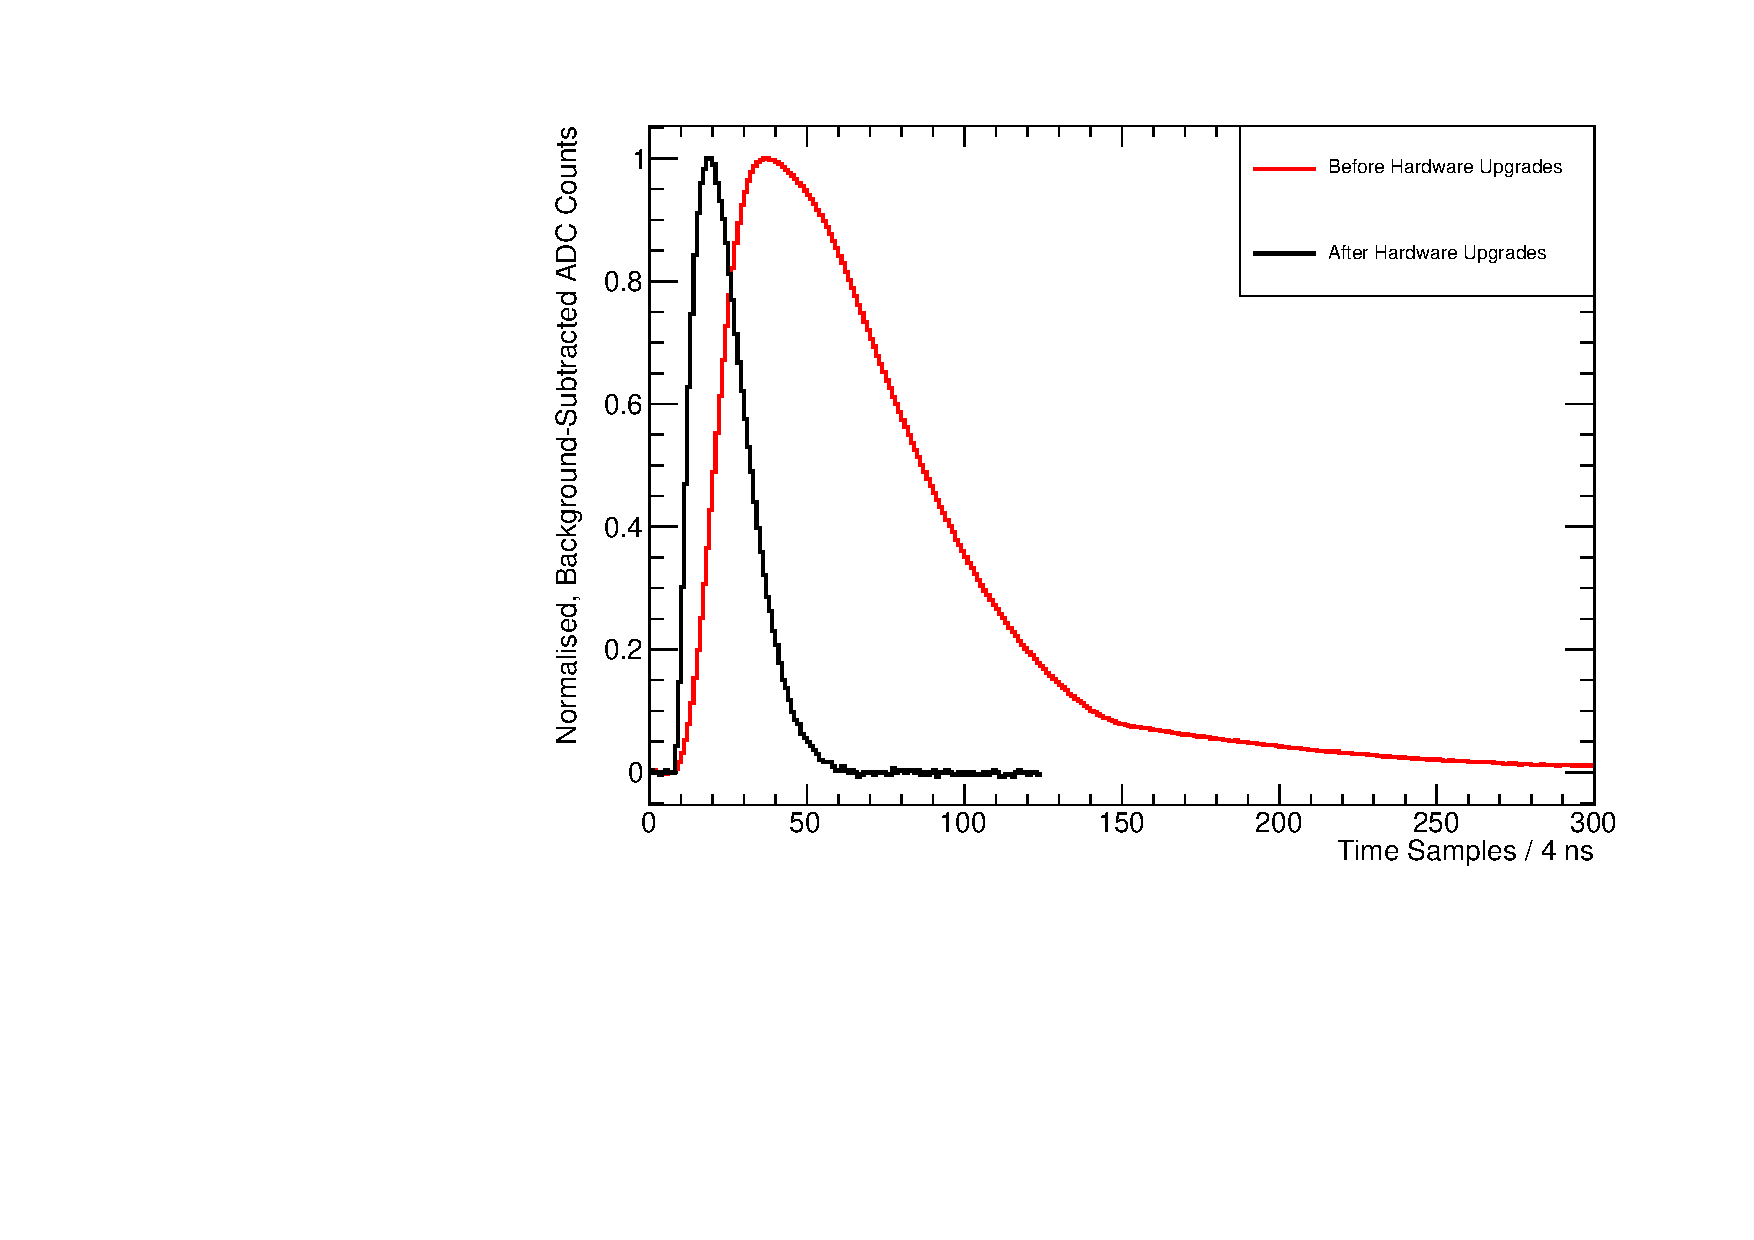
\includegraphics[width=0.8\textwidth]{3_SMELLIEHardware/images/caen_traces_comparison_plot.pdf}
    \caption[Comparison between typical MPU CAEN traces generated by the PQ495 before and after the Summer 2022 hardware upgrades]
    {Comparison between typical MPU CAEN traces generated by the PQ495 before and after the Summer 2022 hardware upgrades. The data before was taken on July 24\textsuperscript{th} 2022, whilst the data after was taken on June 17\textsuperscript{th} 2023. The traces have had their baselines subtracted off, and their peak values normalised to 1.}
    \label{fig:caen_trace_comparison}
\end{figure}

\section{Event Triggering and Data Acquisition}\label{sec:smellie_triggering_daq}
As mentioned in Section~\ref{sec:daq}, it is possible to trigger the SNO+ detector electronics via an external asynchronous trigger, EXTA. Taking data with SMELLIE takes advantage of this capability: instead of waiting for the normal `physics' triggers such as N100 to pick up the event, an EXTA signal can be sent from the firing laser to trigger the detector precisely when a light pulse is within the detector.

\nomenclature{\textbf{NI Unit}}{National Instruments DAQ Unit (for SMELLIE)}
Trigger signal pulses are created by the National Instruments DAQ Unit (the `NI Unit'), in place alongside the rest of the SMELLIE electronics. These trigger pulses are sent to either the PQ's SEPIA controller or the SuperK laser to induce the firing of the relevant laser. If a PQ laser was fired, a trigger pulse is simultaneously sent to TUBii, which after a delay sends an EXTA trigger signal to the MTC/D, which then issues a GT. In contrast, the SuperK has a substantial variation in the emission time of laser light relative to a given driving pulse. Instead of sending the trigger signal to TUBii in parallel to the SuperK laser, a photodiode contained within the SuperK laser system is able to detect any generated light, and from that detection a new trigger signal is sent to TUBii.

A major problem with the handling of the trigger signal delay by TUBii was present throughout the collection of water phase SMELLIE data. This delay was `latched' to the \SI{100}{\MHz} clock present within the electronics of TUBii. As a result, the observed hit times of PMTs in the detector (which are relative to the GT time) was a convolution of the hit times without the latching and a top hat function of width \SI{10}{\ns}.

An example of this effect in action can be seen in Fig.~\ref{fig:smellie_beam_tres_tubii_comparison}. Light from the PQ495 laser was fired through fibre FS007 by E. Turner in June 2018, during the water phase. Looking only at PMTs that were hit in the beamspot, defined here as PMTs with $\alpha<\ang{3}$, the trigger times can be fit to the convolution of a Gaussian with a \SI{10}{\ns} top hat.

\begin{figure}
    \centering
    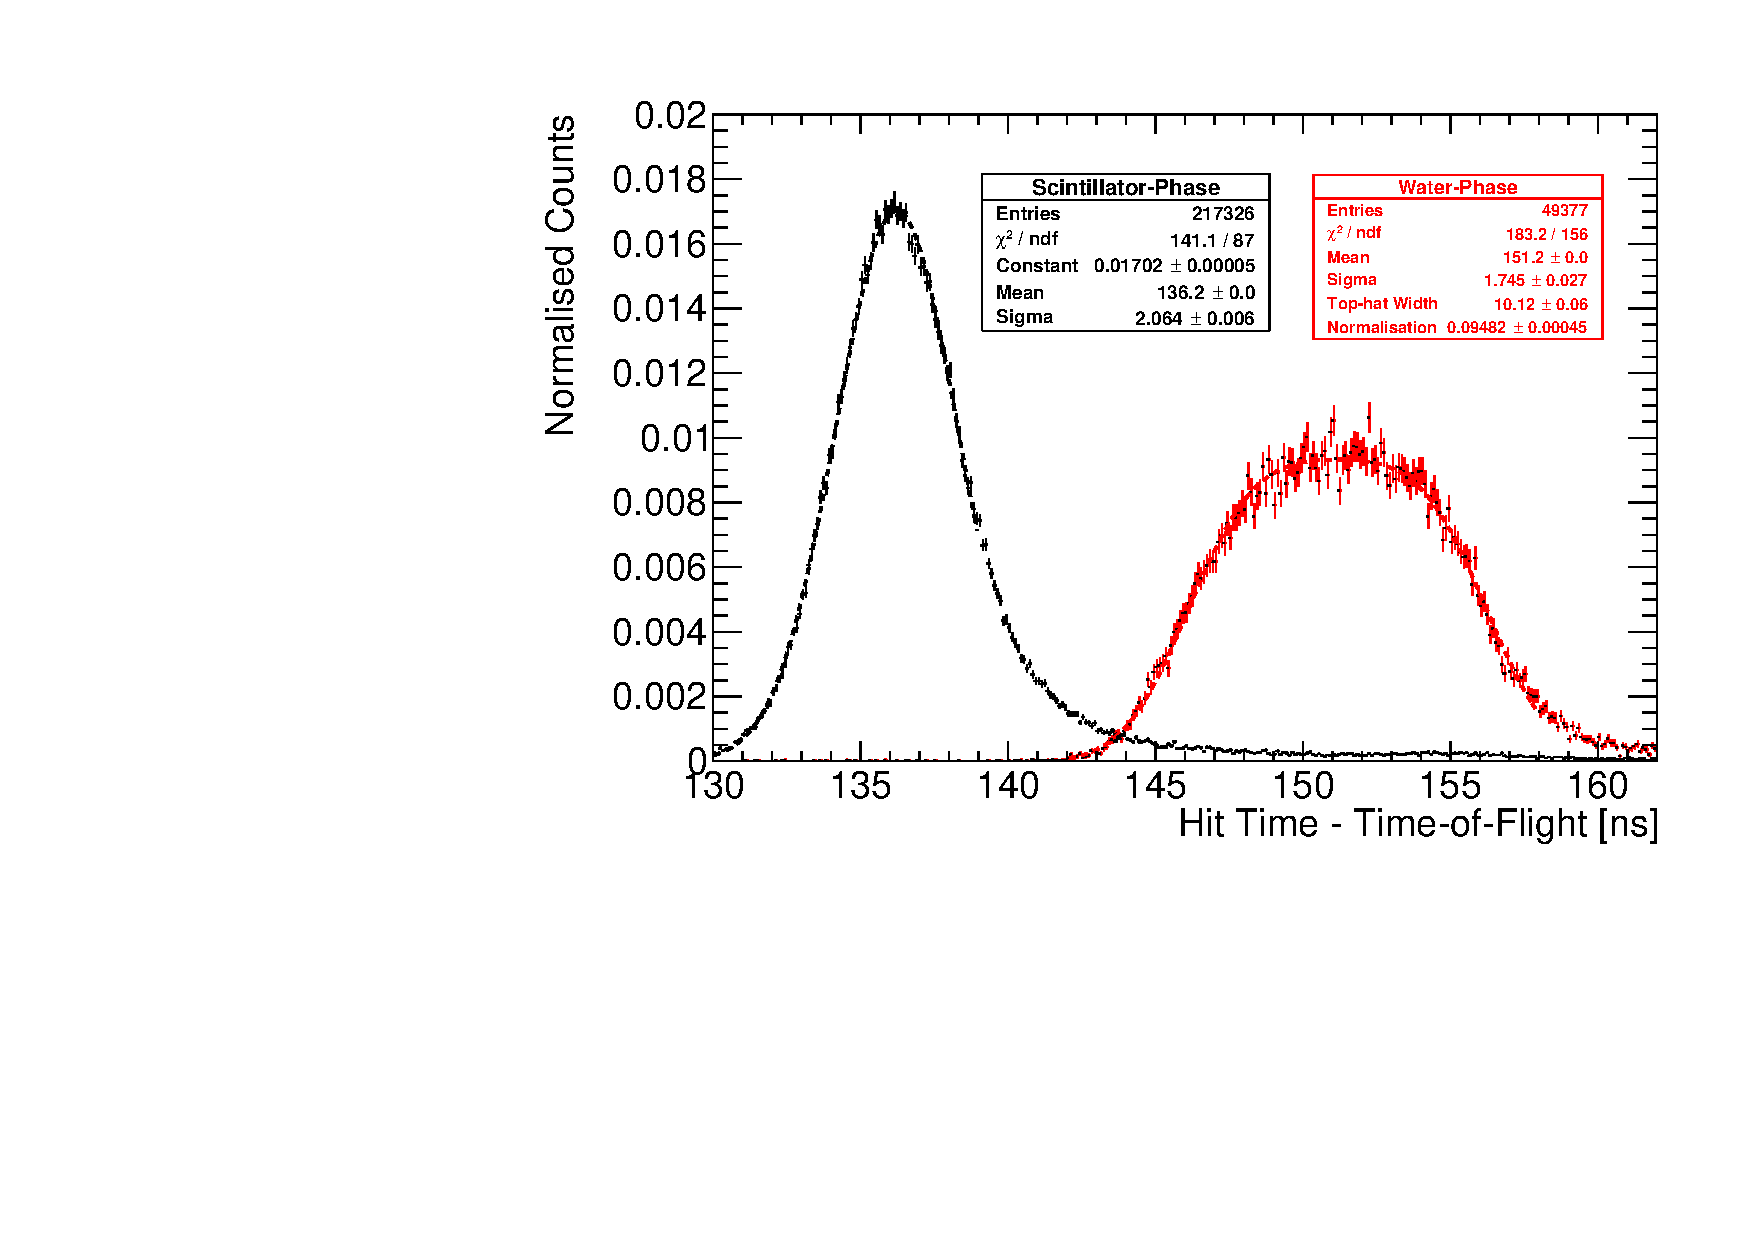
\includegraphics[width=0.8\textwidth]{3_SMELLIEHardware/images/time_plots_comparison_114018_vs_302634_FS007_nice.pdf}
    \caption[Comparison of observed hit times in beamspot before and after TUBii firmware update]
    {Comparison of observed hit times in beamspot for laser PQ495 through fibre FS007, before and after T. Zummo's firmware update to TUBii. The initial data was taken by E. Turner June 20\textsuperscript{th} 2018 during the water phase, whilst the data post-fix was taken by myself on June 24\textsuperscript{th} 2023 during the scintillator phase. The peak of the former is fit to the convolution of a Gaussian with a top-hat function, whilst the latter is just fit with a Gaussian function.}
    \label{fig:smellie_beam_tres_tubii_comparison}
\end{figure}

During the partial fill phase, Tony Zummo updated the firmware of TUBii so that this latching would no longer occur, and the arrival times to the MTC/D were truly asynchronous to any clocks. The results are also shown in Fig.~\ref{fig:smellie_beam_tres_tubii_comparison}: notice how the width of the peak is now much sharper. This width is determined by the TTS of the hit PMTs, with the width of the PQ495 timing pulse being a subdominant effect.

Because this fix to TUBii was not in place until after all water phase data taking had been completed, any analysis of SMELLIE data from the water phase had to contend with this \SI{10}{\ns} trigger `jitter'. Fortunately, this jitter was global to all hit times of a given event, so if measured a correction could be made.

In this thesis, two similar approaches are used to measure the event-by-event emission time $t_{\mathrm{emm}}$, the time at which laser light first emanates from the fibre in a given event. In both, the calibrated hit times of PMTs within the beamspot $t_{\mathrm{hit}}$ have the time-of-flight of light travelling from the fibre to the given PMT, $t_{\mathrm{TOF}}$ subtracted. $t_{\mathrm{TOF}}$ is calculated by using the ``Light Path Calculator'' algorithm developed within \texttt{RAT}. In one method, used both within the analysis work of E. Turner~\cite{turnerMeasurementScatteringCharacteristics2022} % cite anyone else?
and in Chapter~\ref{chap:beam_profiling} of this thesis, $t_{\mathrm{emm}}$ is measured as the second-earliest value of $t_{\mathrm{hit}}-t_{\mathrm{TOF}}$ in the beamspot. This method, called the ``$t_{\mathrm{emm}} = t_{2}$'' approach, skips the earliest event in the beamspot to be robust to noise hits.

Alternatively, in the ``$t_{\mathrm{emm}} = t_{\mathrm{med}}$'' approach, the median value of $t_{\mathrm{hit}}-t_{\mathrm{TOF}}$ in the beamspot is used. We shall see in Chapter~\ref{chap:smellie_analysis} that using $t_{2}$ has a bias as a function of the number of hits in the beamspot in a given event, whereas $t_{\mathrm{med}}$ does not.

This event-by-event approach to reconstructing $t_{\mathrm{emm}}$ is only necessary when the trigger system has unresolved problems. Because of the fix to the TUBii firmware, data taken using the PQ lasers during the scintillator phase did not in theory require using either of the $t_{\mathrm{emm}}$ reconstruction methods described above. However, for the SuperK laser a new problem was made clear. In Fig.~\ref{fig:smellie_superk_double_peaks} one can see the hit times of beamspot PMTs for SuperK light of wavelengths in the interval $[490,500]\;\si{\nm}$ from fibre FS125, taken on June 17\textsuperscript{th} 2023. % COMPLETE!
A clear double-peaked structure can be seen. Also shown on the plot is the distribution of $t_{2}$ values. If the laser light were being emitted in two pulses for a given event, then it would be expected to see only one bump in this distribution. However, the shape of the $t_{2}$ is clearly bimodal in a manner matching that of the overall timing distribution: this indicates that the actual emission times of light from the fibre can come at two different times relative to the GT time.

\begin{figure}
    \centering
    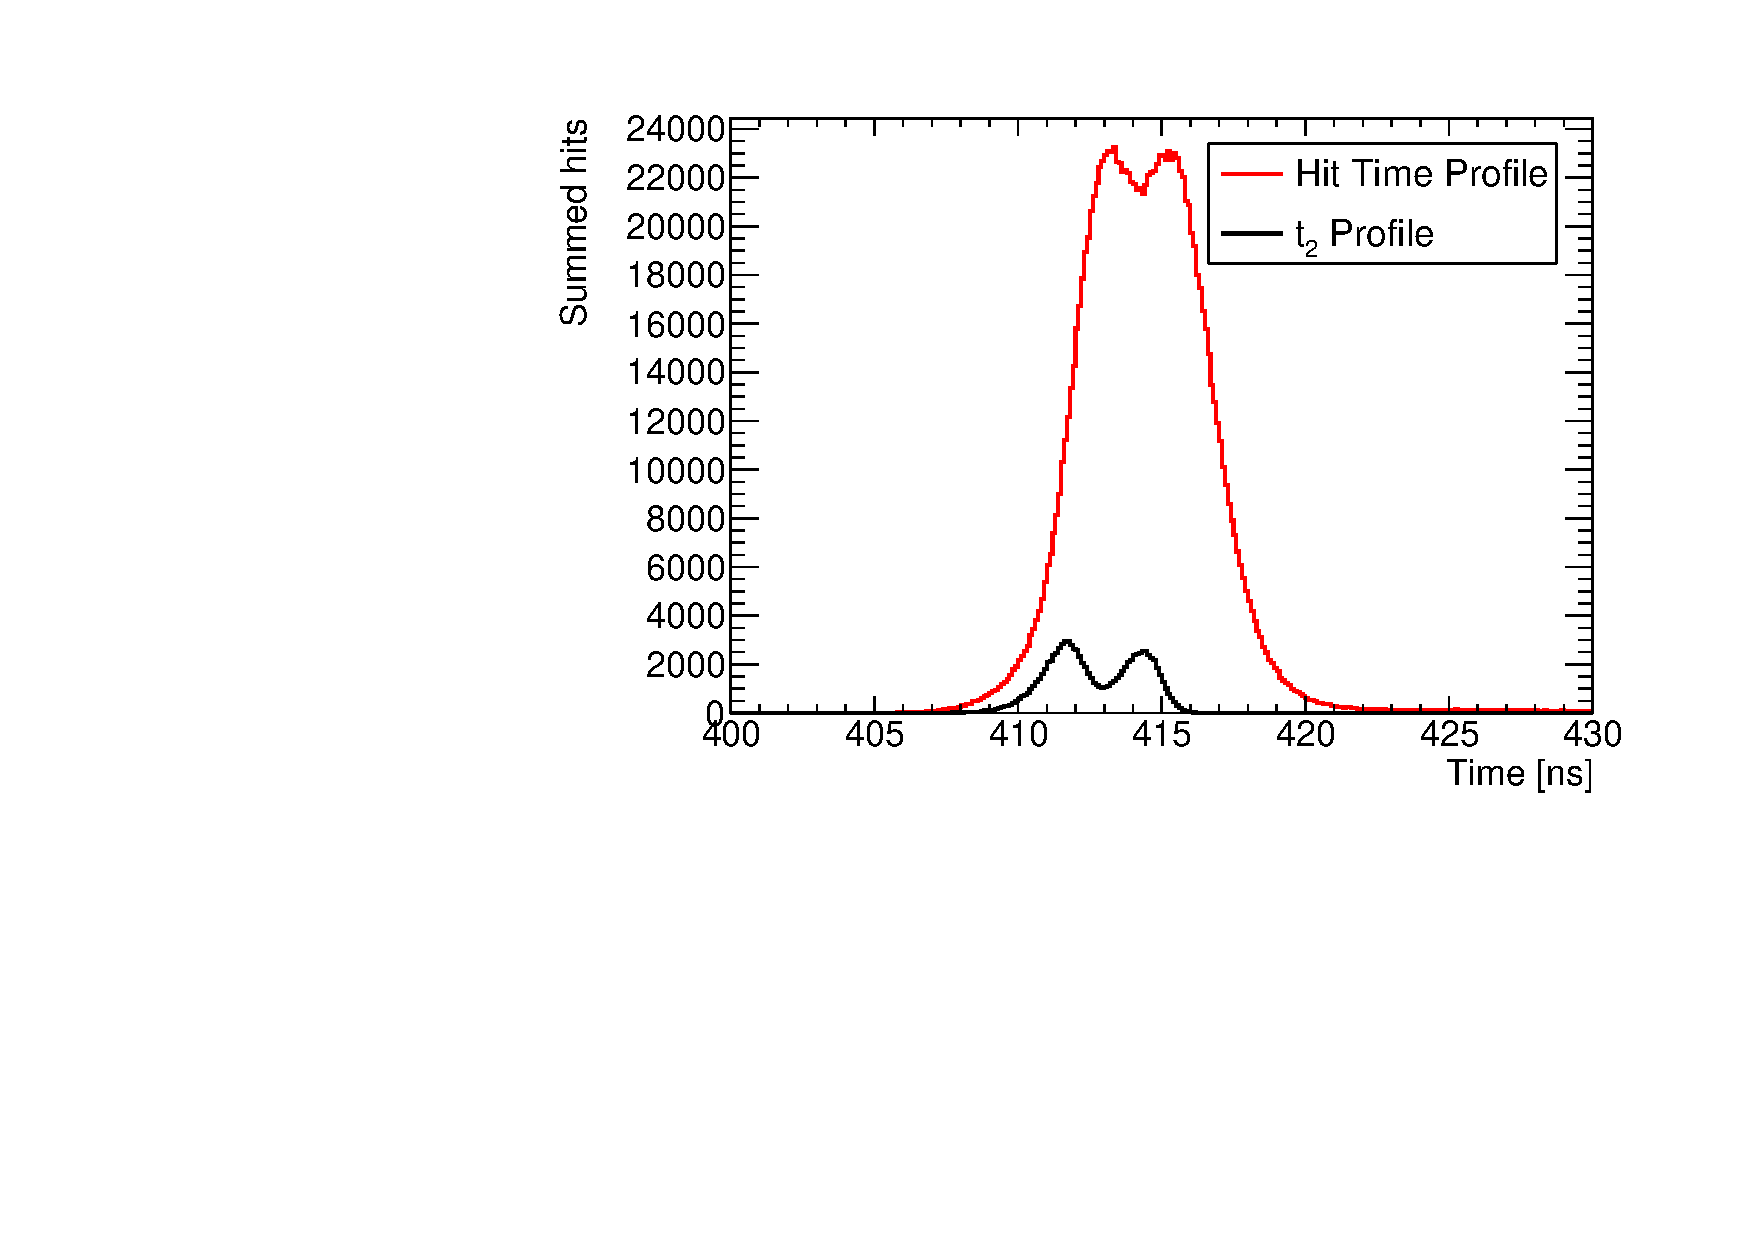
\includegraphics[width=0.8\textwidth]{3_SMELLIEHardware/images/time_t2_plot_310303_SK495_FS125.pdf}
    \caption[]{Hit time and $t_{2}$ distributions for a subrun of SMELLIE data taken with the SuperK laser in the $[490,500]\;\si{\nm}$ range through fibre FS125 on June 17\textsuperscript{th} 2023. The double-peaked structure is clear in both distributions.}
    \label{fig:smellie_superk_double_peaks}
\end{figure}

The origin of this double-peaked structure for SuperK events remains unresolved. However, the fact that events from the PQ lasers do not see this effect indicates that the issue likely lies somewhere in the part of the triggering system unique to the SuperK laser. For work within this thesis, it was decided to continue to use an event-by-event approach to $t_{\mathrm{emm}}$ for data from all phases and lasers, to ensure consistency.

% TALK ABOUT PULSEGT????

% \begin{itemize}
%     \item Describe the existing hardware, post-upgrade made in Summer 2022. For pre-upgrade hardware, can simply cite previous SMELLIE theses. This includes the path of light into the detector, as well as the path of the trigger signal.
%     \item Make sure to mention explicitly these upgrades: Tony Zummo's fix to the TUBii trigger logic, as well as the addition of the VFA, updated MPU, and modified trigger window. Make sure to motivate why these updates were made.
% \end{itemize}
% [7 pages]
\section{Software for SMELLIE Data-taking}
The process of taking data with SMELLIE is largely automated. The user begins by deciding on the settings --- the number of laser pulses and their frequency, as well as which fibre, laser, wavelength, intensity, and attenuation (if relevant) --- that will be used for each subrun. One run of SMELLIE data taking can have an arbitrary number of subruns within it, each with their own setting. This is organised into a ``run plan'' \texttt{JSON} file for that run, and uploaded to a central CouchDB server for storage.

To begin data taking, ORCA is used to put the DAQ into a `SMELLIE' run type, which disables almost all the usual `Physics' triggers such as N100 and N20. The only triggers still masked into the MTC/D are:
\begin{itemize}
    \item EXTA: This is needed to capture the trigger signals sent from SMELLIE.
    \item ESUMHI: This residual physics trigger is kept in with a high threshold, to capture any high-\texttt{nhit} events not coming from SMELLIE, e.g. if a supernova were to go off whilst SMELLIE data taking was occurring.
    \item PULSEGT: This is a special trigger that fires at a rate of \SI{50}{\Hz} independent of all other systems. With this trigger, the noise rate can be calculated on a run-by-run basis for each channel.
\end{itemize}
The noise rates derived from the PULSEGT triggers are automatically calculated during the processing of runs, and are stored in \texttt{RATDB} tables. As mentioned in Section~\ref{sec:ev_simulation}, \texttt{RAT} can use these tables to replicate the noise levels in each PMT when generating simulations to match data. When performing analysis on SMELLIE data, only events from an EXTA trigger are usually considered.

With ORCA, one can then load in any run plan already uploaded to the CouchDB server, and then execute it. ORCA then sends commands describing the instructions laid out in the run plan to a server running on a computer called SNODROP, which is housed in the same pair of electronic racks as the rest of the SMELLIE hardware. This server converts these high-level commands into the low level instructions understood by the specific pieces of SMELLIE hardware needed to actually send the correct number of pulses of laser light of the right wavelength and intensity through the correct fibre. Details of the integration of SMELLIE with ORCA can be found in~\cite{jonesFutureSearchesRare2016}

Whilst SMELLIE data is being taken, a ``run description'' \texttt{JSON} file is generated and then uploaded to the SMELLIE CouchDB server, describing the settings of the SMELLIE run actually executed. This differs from the run plan slightly in two main ways: firstly, the same run plan can be run on multiple occasions. However, a run description file is associated to exactly one run of data that was actually taken. Secondly, if a SMELLIE run was terminated early either by the detector operator, or from a hardware problem, the run description file will correctly show only the subruns that were actually performed. The code repository used in all SMELLIE analysis has been updated by myself to use a given run description file in concert with the associated SMELLIE data file, so that the subrun-level metadata can be known during analysis.


% \begin{itemize}
%     \item Can be brief here! Little has changed since previous theses, so can mostly just summarise and cite.
%     \item Server running on SNODROP machine, which converts high-level commands into low-level ones that the hardware can interpret.
%     \item Run plan files written in JSON handed to ORCA which then sends relevant commands to SNODROP which fires as appropriate.
%     \item Operator interacts with ORCA to perform SMELLIE calibration runs.
%     \item After SMELLIE data taken, run description file created, containing metadata about the run conditions, used in analysis.
% \end{itemize}
% [2 pages]

% MAYBE DO NOT INCLUDE SMELLIE COMMISSIONING SECTION????

% \section[Commissioning SMELLIE in the Scintillator Phase]{Commissioning SMELLIE in the\\ Scintillator Phase}

% {
% \color{blue}
% \begin{itemize}
%     \item Explain why commissioning of SMELLIE is needed: Need to confirm that SMELLIE is working as expected; determine intensity "set-points" for different use cases.
%     \item Commissioning originally performed by Esther and JeffL back in the water phase; explain why this needed to be re-done for both the scintillator phase and after the hardware upgrades.
%     \item No need to describe the Tesseract in detail here - that can be in Jeff L's thesis. But, I do want to show the results of both commissioning campaigns in scintillator-fill, one before the new hardware was added, and one after.
% \end{itemize}
% [5 pages]
% [15 PAGES TOTAL]
% }